%\appendix
\chapter{BDT plots}
\label{sec:appBDTplots}


\subsubsection{Low mass splittings}
\begin{figure}[H]
    \centering
    \begin{subfigure}[t!]{0.49\textwidth}
        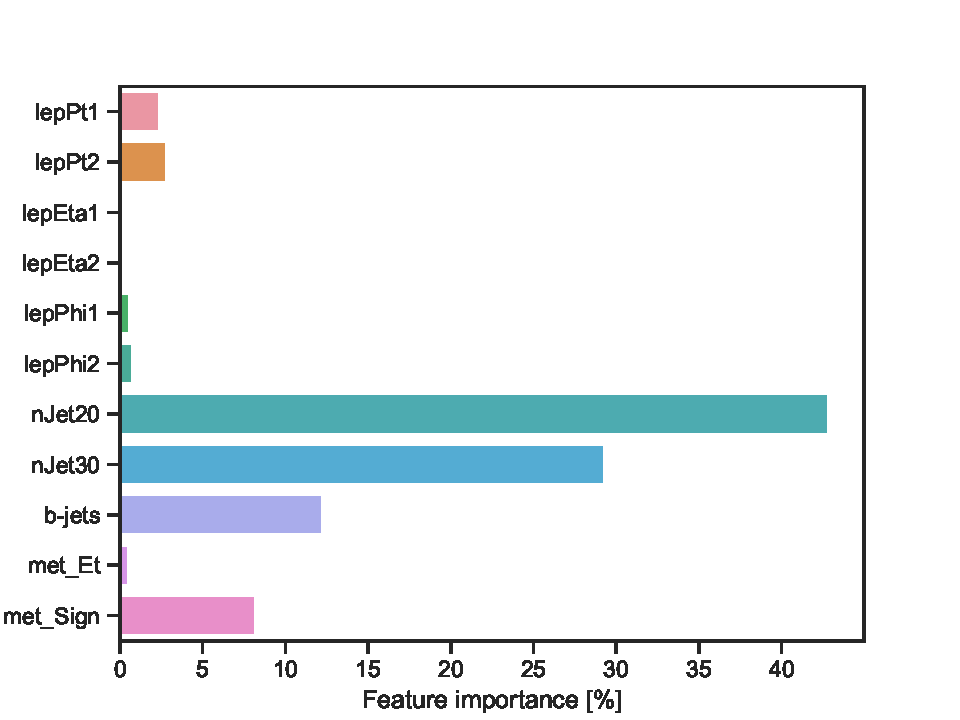
\includegraphics[width = \textwidth]{Figures/SlepSlep/ML/BDT/Low_level/Low/featureImportance.pdf}
        \caption{}
        \label{fig:featSlepslepLow}
    \end{subfigure}
    \begin{subfigure}[t!]{0.49\textwidth}
        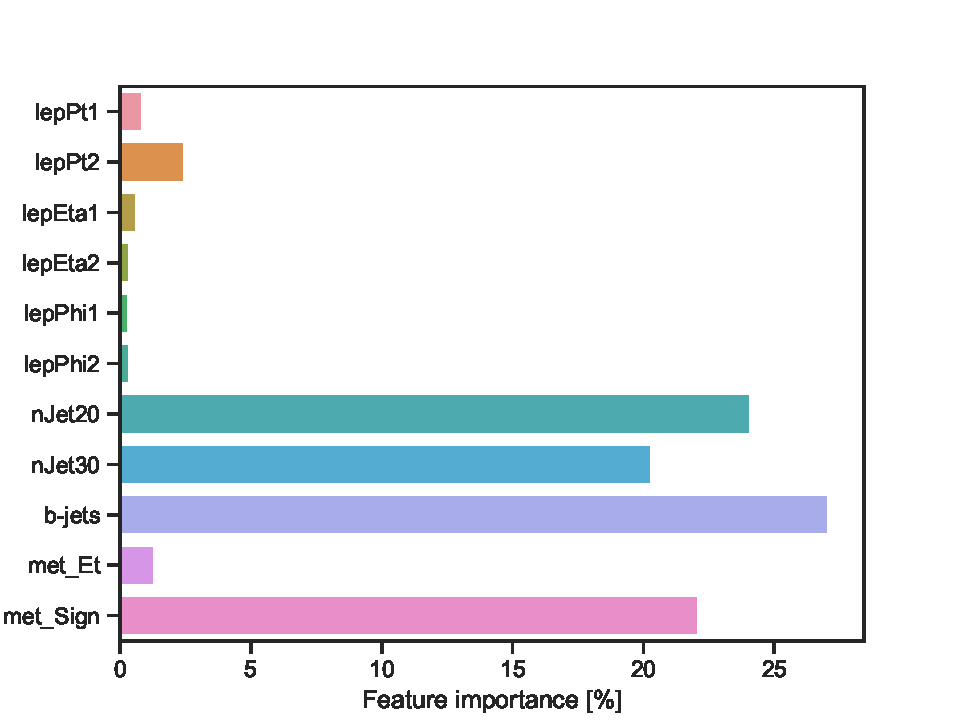
\includegraphics[width = \textwidth]{Figures/SlepSnu/BDT/Low_level/Low/featureImportance.pdf}
        \caption{}
        \label{fig:featSlepsnuLow}
    \end{subfigure}
    \begin{subfigure}[t!]{0.49\textwidth}
        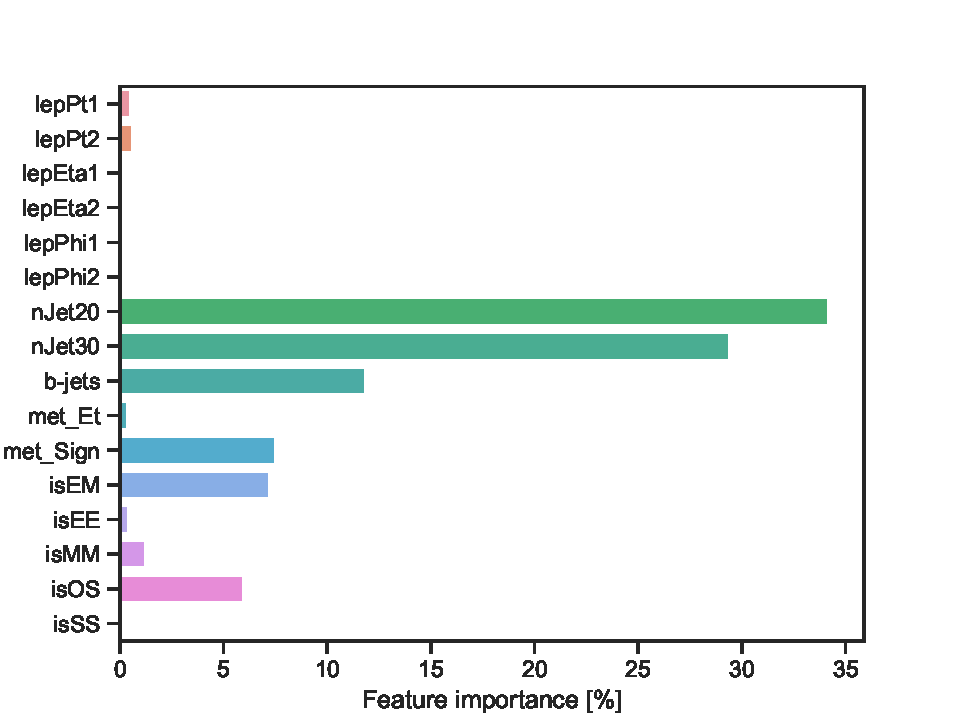
\includegraphics[width = \textwidth]{Figures/WW/BDT/Low_level/Low/featureImportance.pdf}
        \caption{}
        \label{fig:featWWLow}
    \end{subfigure}
    \begin{subfigure}[t!]{0.49\textwidth}
        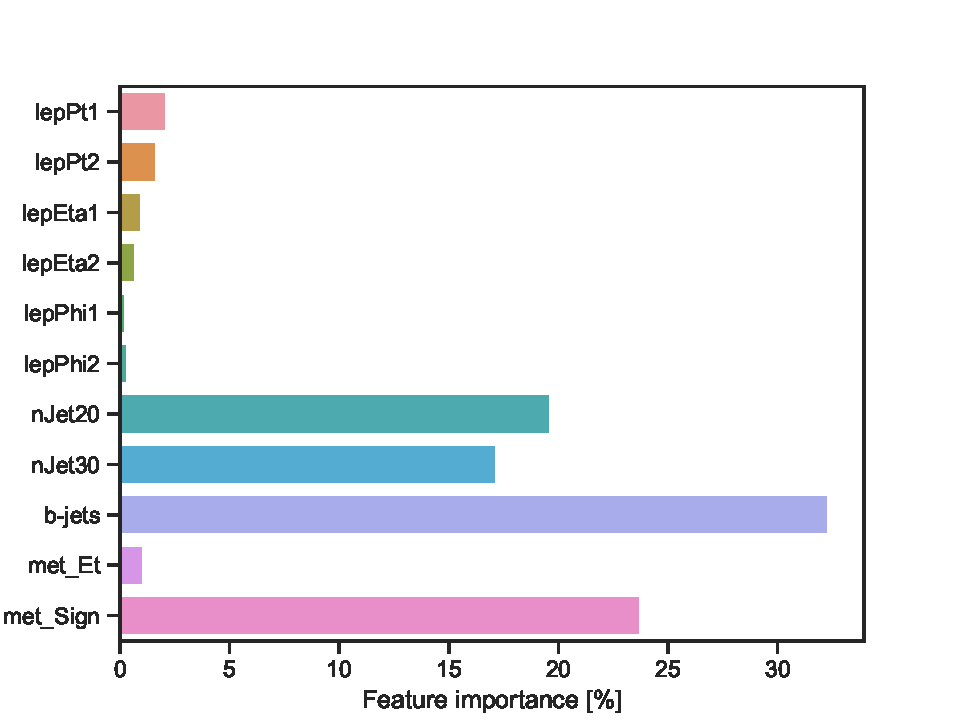
\includegraphics[width = \textwidth]{Figures/Mono_Z/ML/BDT/Low_level/Low/featureImportance.pdf}
        \caption{}
        \label{fig:featMonoZLow}
    \end{subfigure}
    \caption{}
    \label{fig:Non}
\end{figure}

\begin{figure}[H]
    \centering
    \begin{subfigure}[t!]{0.49\textwidth}
        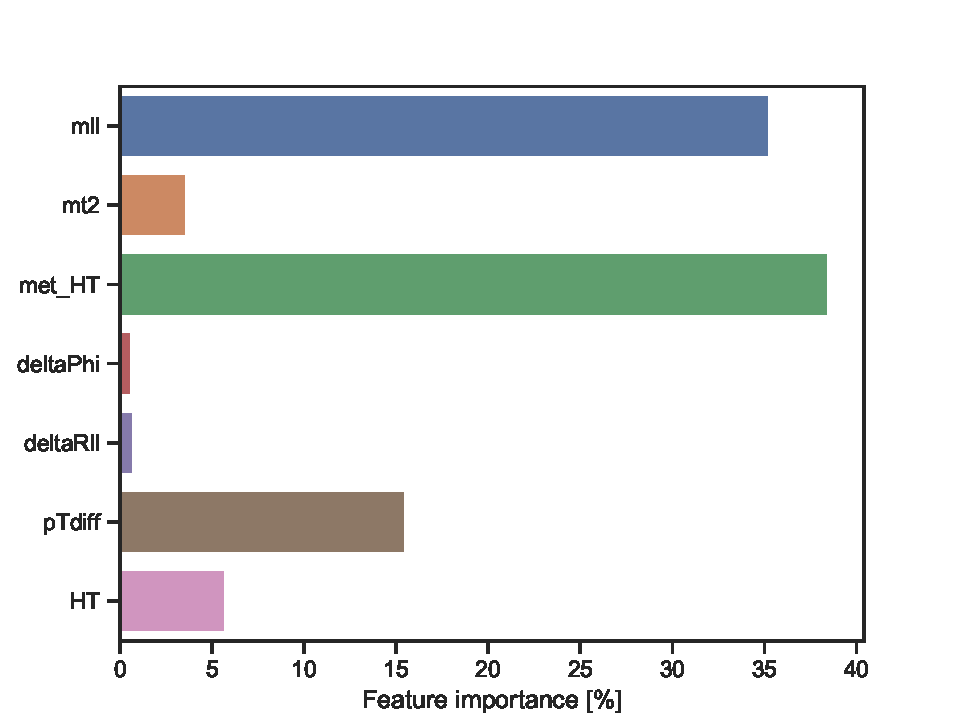
\includegraphics[width = \textwidth]{Figures/SlepSlep/ML/BDT/High_level/Low/featureImportance.pdf}
        \caption{}
        \label{fig:featSlepslepLow}
    \end{subfigure}
    \begin{subfigure}[t!]{0.49\textwidth}
        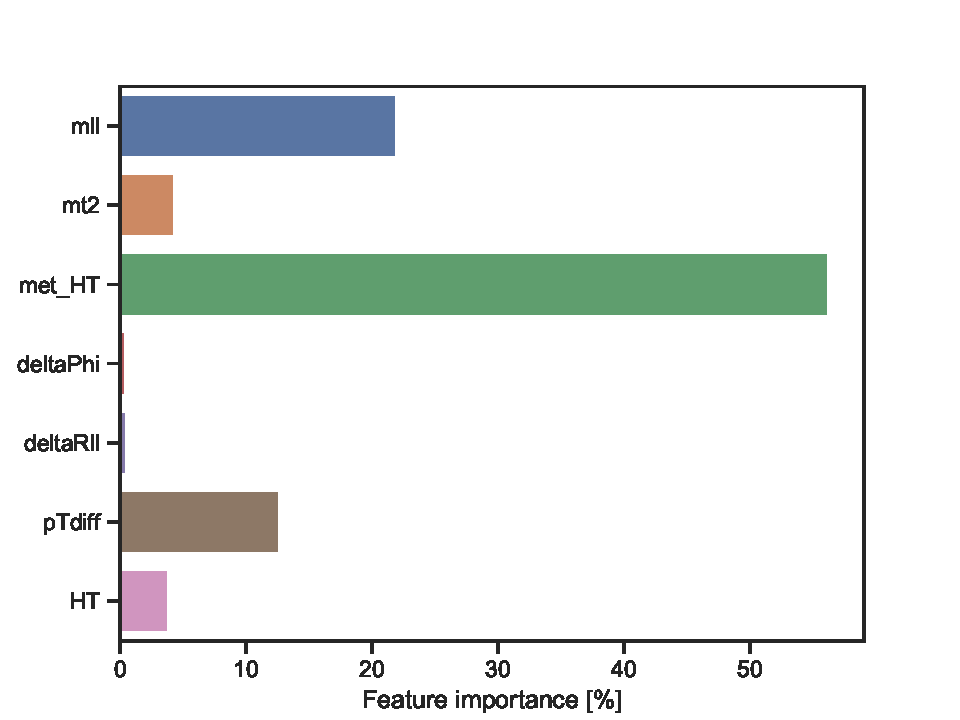
\includegraphics[width = \textwidth]{Figures/SlepSnu/BDT/High_level/Low/featureImportance.pdf}
        \caption{}
        \label{fig:featSlepsnuLow}
    \end{subfigure}
    \begin{subfigure}[t!]{0.49\textwidth}
        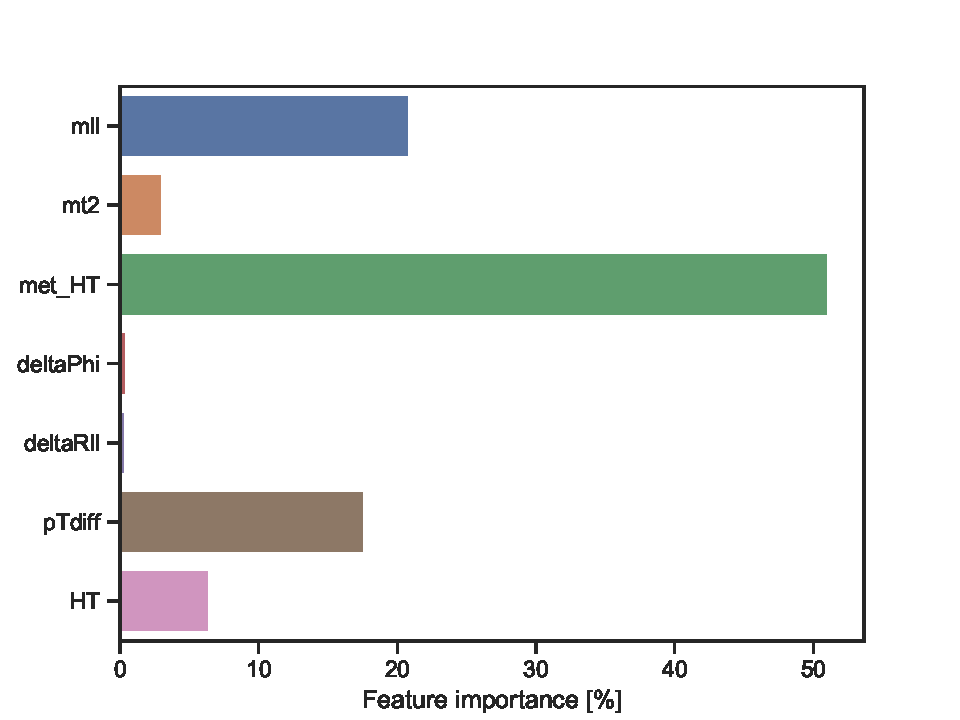
\includegraphics[width = \textwidth]{Figures/WW/BDT/High_level/Low/featureImportance.pdf}
        \caption{}
        \label{fig:featWWLow}
    \end{subfigure}
    \begin{subfigure}[t!]{0.49\textwidth}
        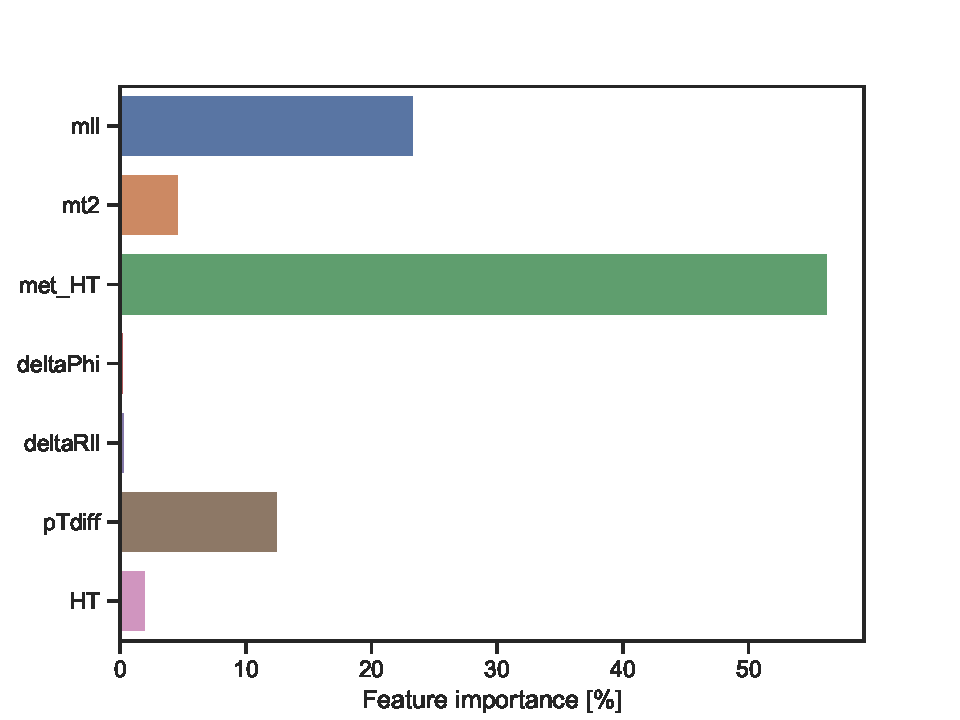
\includegraphics[width = \textwidth]{Figures/Mono_Z/ML/BDT/High_level/Low/featureImportance.pdf}
        \caption{}
        \label{fig:featMonoZLow}
    \end{subfigure}
    \caption{}
    \label{fig:Non}
\end{figure}

\begin{figure}[H]
    \centering
    \begin{subfigure}[t!]{0.49\textwidth}
        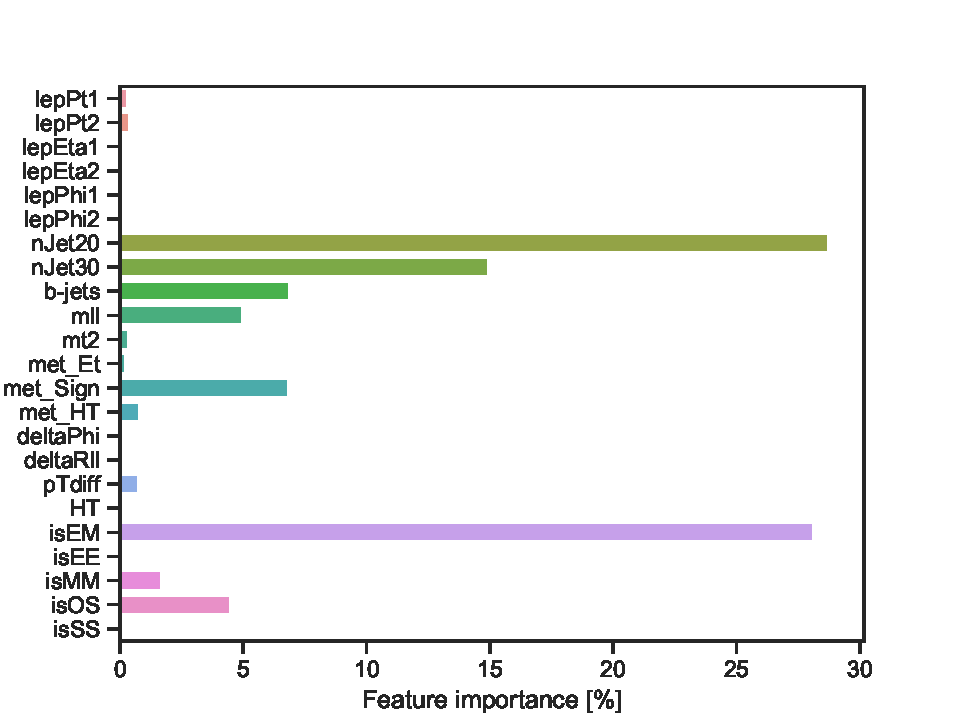
\includegraphics[width = \textwidth]{Figures/SlepSlep/ML/BDT/All_level/Low/featureImportance.pdf}
        \caption{}
        \label{fig:featSlepslepLow}
    \end{subfigure}
    \begin{subfigure}[t!]{0.49\textwidth}
        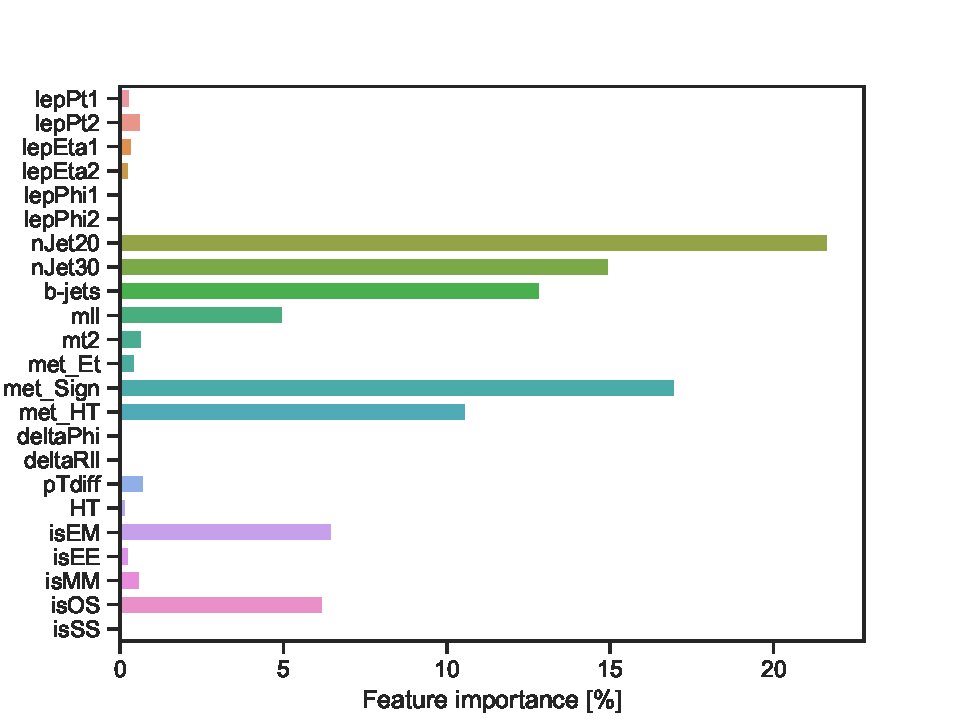
\includegraphics[width = \textwidth]{Figures/SlepSnu/BDT/All_level/Low/featureImportance.pdf}
        \caption{}
        \label{fig:featSlepsnuLow}
    \end{subfigure}
    \begin{subfigure}[t!]{0.49\textwidth}
        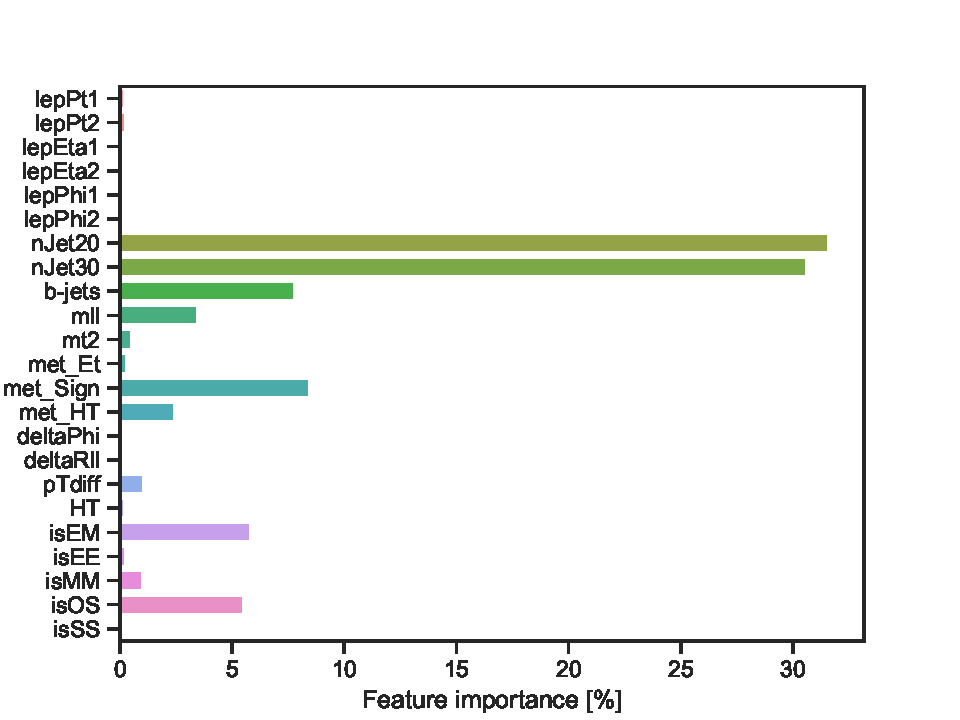
\includegraphics[width = \textwidth]{Figures/WW/BDT/All_level/Low/featureImportance.pdf}
        \caption{}
        \label{fig:featWWLow}
    \end{subfigure}
    \begin{subfigure}[t!]{0.49\textwidth}
        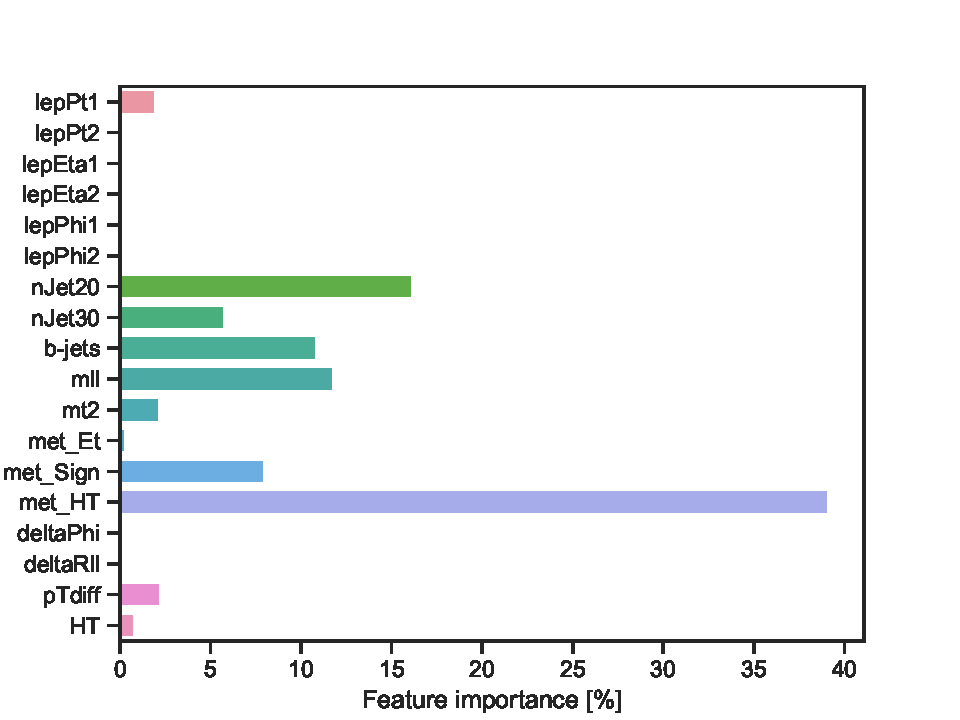
\includegraphics[width = \textwidth]{Figures/Mono_Z/ML/BDT/All_level/Low/featureImportance.pdf}
        \caption{}
        \label{fig:featMonoZLow}
    \end{subfigure}
    \caption{}
    \label{fig:Non}
\end{figure}

\begin{figure}[H]
    \centering
    \begin{subfigure}[t!]{0.49\textwidth}
        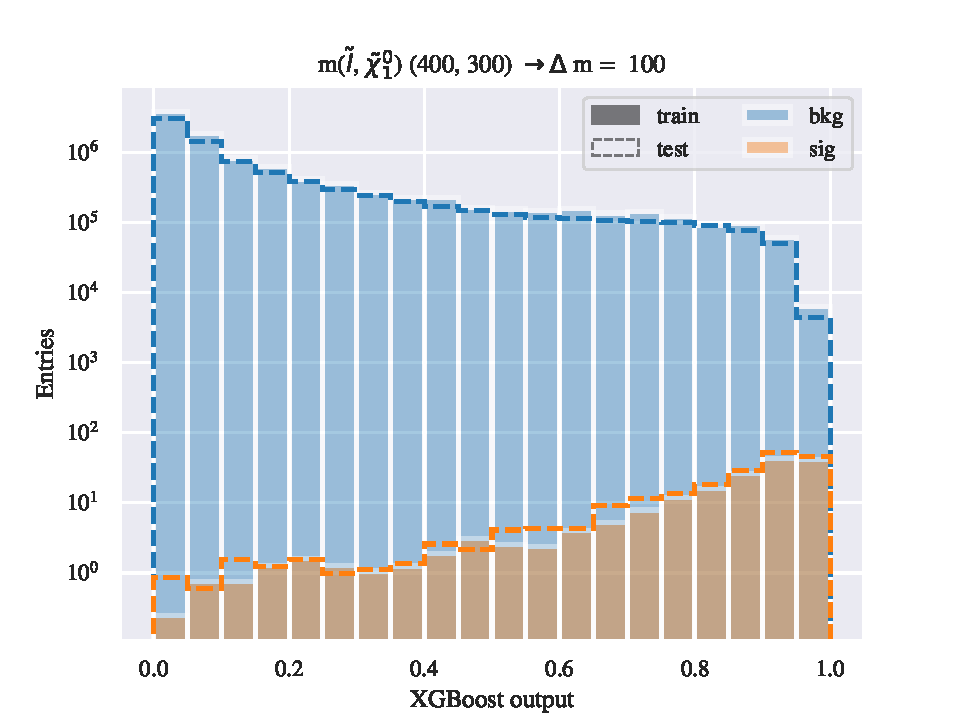
\includegraphics[width = \textwidth]{Figures/SlepSlep/ML/BDT/High_level/Low/scaled_train_test_395984.pdf}
        \caption{}
        \label{fig:traintestscaledBDTSlepslepLow}
    \end{subfigure}
    \begin{subfigure}[t!]{0.49\textwidth}
        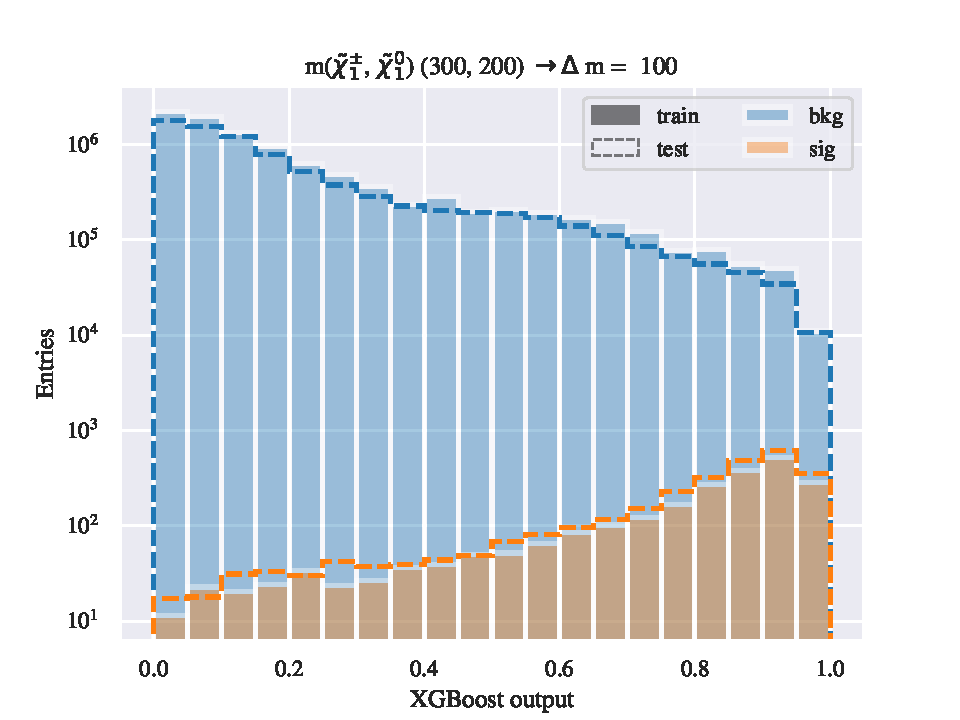
\includegraphics[width = \textwidth]{Figures/SlepSnu/BDT/Low_level/Low/scaled_train_test_397115.pdf}
        \caption{}
        \label{fig:traintestscaledBDTSlepsnuLow}
    \end{subfigure}
    \begin{subfigure}[t!]{0.49\textwidth}
        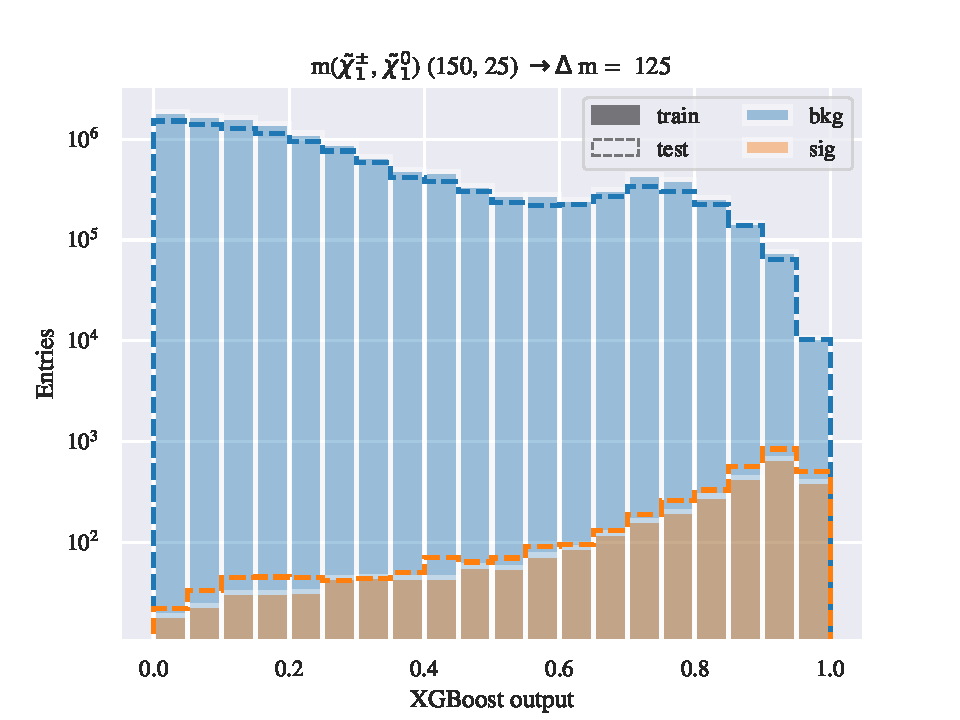
\includegraphics[width = \textwidth]{Figures/WW/BDT/Low_level/Low/scaled_train_test_395268.pdf}
        \caption{}
        \label{fig:traintestscaledBDTWWLow}
    \end{subfigure}
    \begin{subfigure}[t!]{0.49\textwidth}
        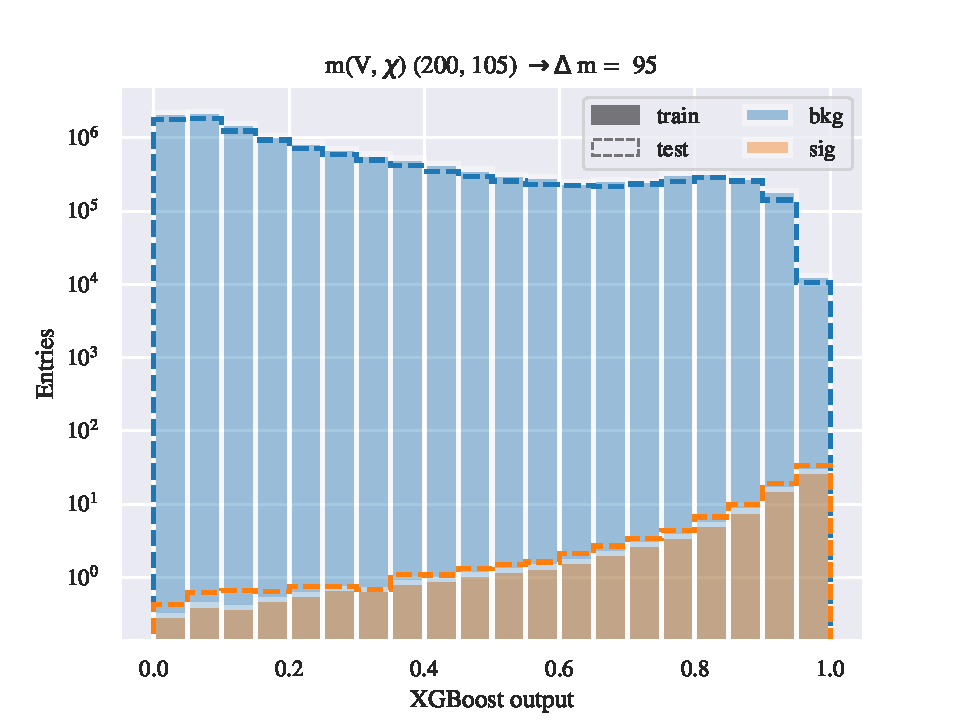
\includegraphics[width = \textwidth]{Figures/Mono_Z/ML/BDT/Low_level/Low/scaled_train_test_310604.pdf}
        \caption{}
        \label{fig:traintestscaledBDTMonoZLow}
    \end{subfigure}
    \caption{}
    \label{fig:Non}
\end{figure}

\subsubsection{Intermediate mass splittings}
\begin{figure}[H]
    \centering
    \begin{subfigure}[t!]{0.49\textwidth}
        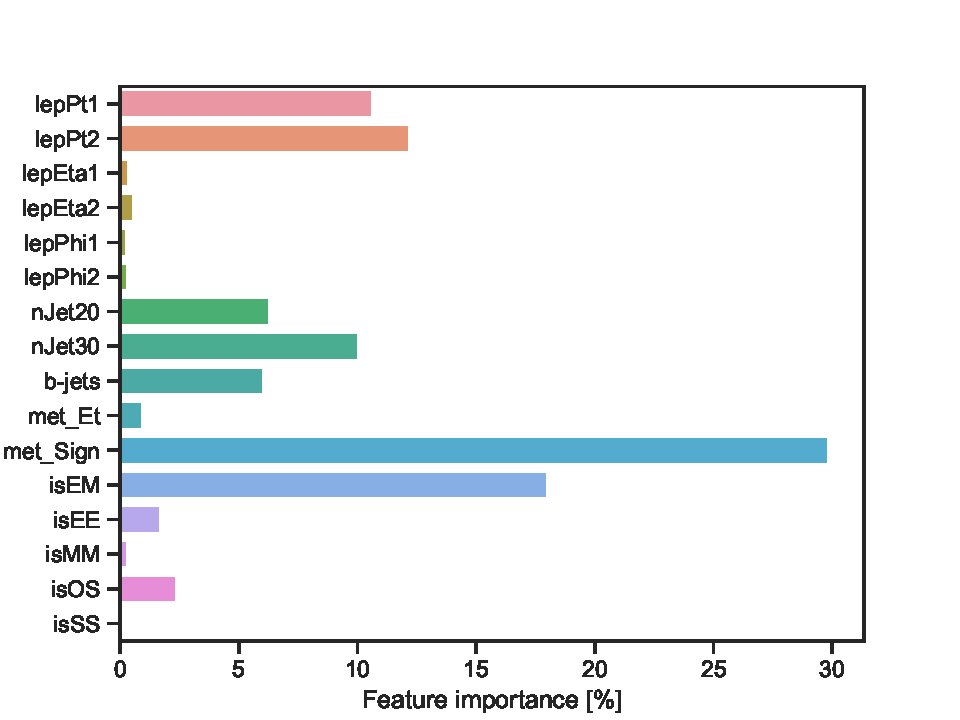
\includegraphics[width = \textwidth]{Figures/SlepSlep/ML/BDT/Low_level/Inter/featureImportance.pdf}
        \caption{}
        \label{fig:featSlepslepLow}
    \end{subfigure}
    \begin{subfigure}[t!]{0.49\textwidth}
        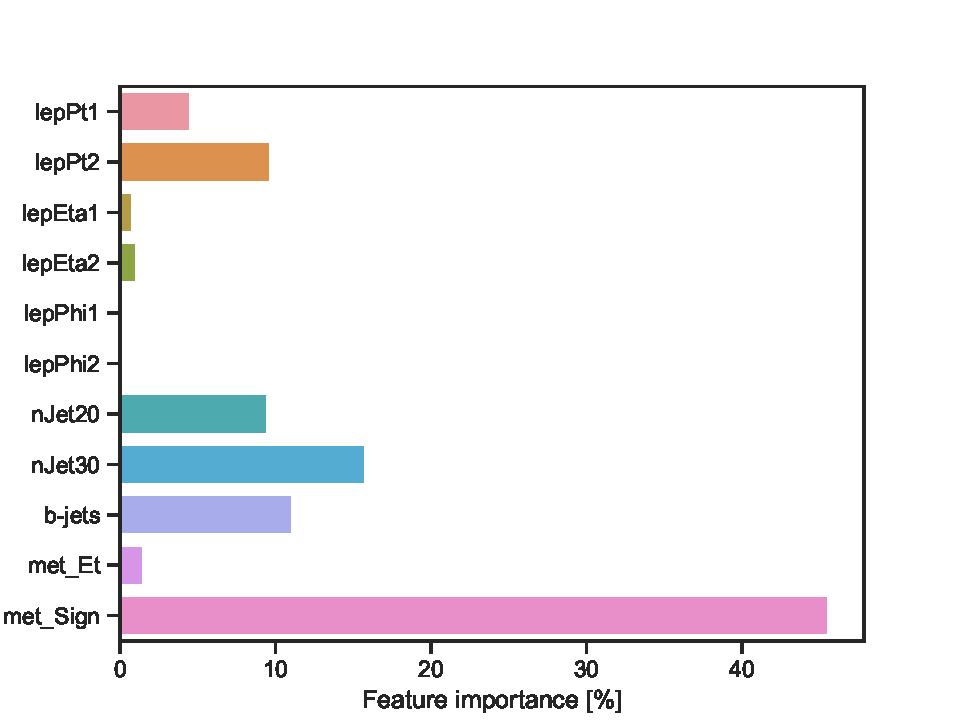
\includegraphics[width = \textwidth]{Figures/SlepSnu/BDT/Low_level/Inter/featureImportance.pdf}
        \caption{}
        \label{fig:featSlepsnuLow}
    \end{subfigure}
    \begin{subfigure}[t!]{0.49\textwidth}
        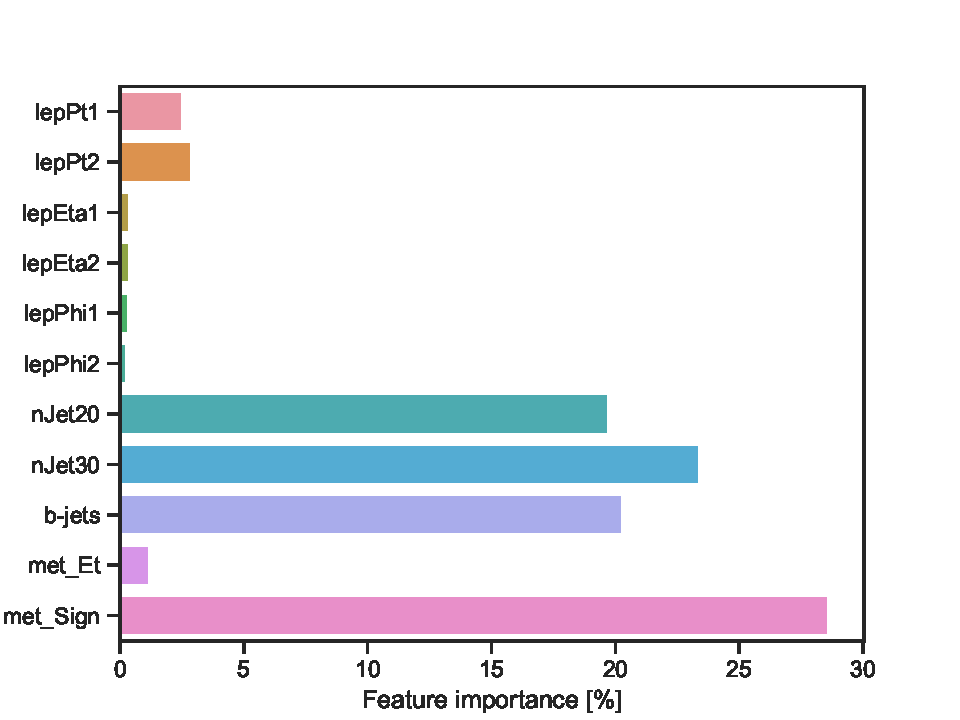
\includegraphics[width = \textwidth]{Figures/WW/BDT/Low_level/Inter/featureImportance.pdf}
        \caption{}
        \label{fig:featWWLow}
    \end{subfigure}
    \begin{subfigure}[t!]{0.49\textwidth}
        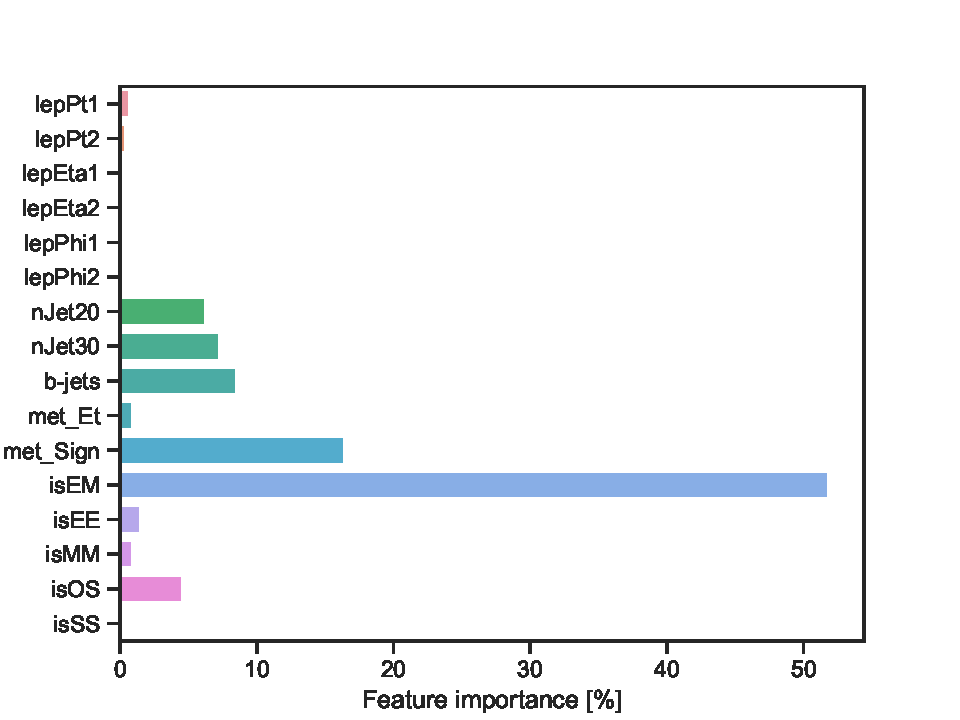
\includegraphics[width = \textwidth]{Figures/Mono_Z/ML/BDT/Low_level/Inter/featureImportance.pdf}
        \caption{}
        \label{fig:featMonoZLow}
    \end{subfigure}
    \caption{}
    \label{fig:Non}
\end{figure}

\begin{figure}[H]
    \centering
    \begin{subfigure}[t!]{0.49\textwidth}
        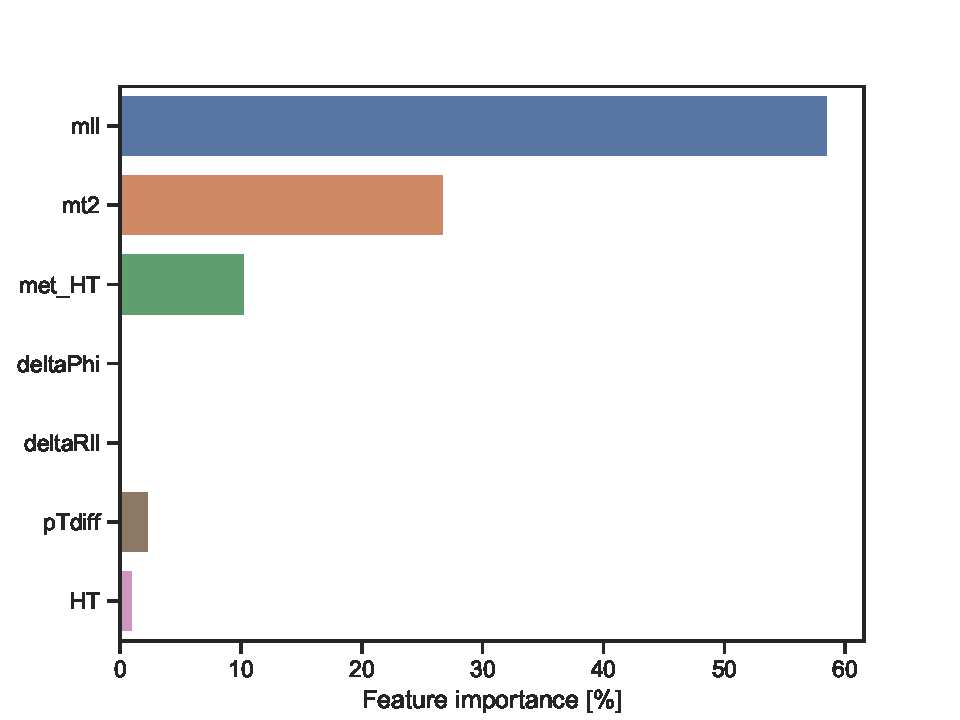
\includegraphics[width = \textwidth]{Figures/SlepSlep/ML/BDT/High_level/Inter/featureImportance.pdf}
        \caption{}
        \label{fig:featSlepslepLow}
    \end{subfigure}
    \begin{subfigure}[t!]{0.49\textwidth}
        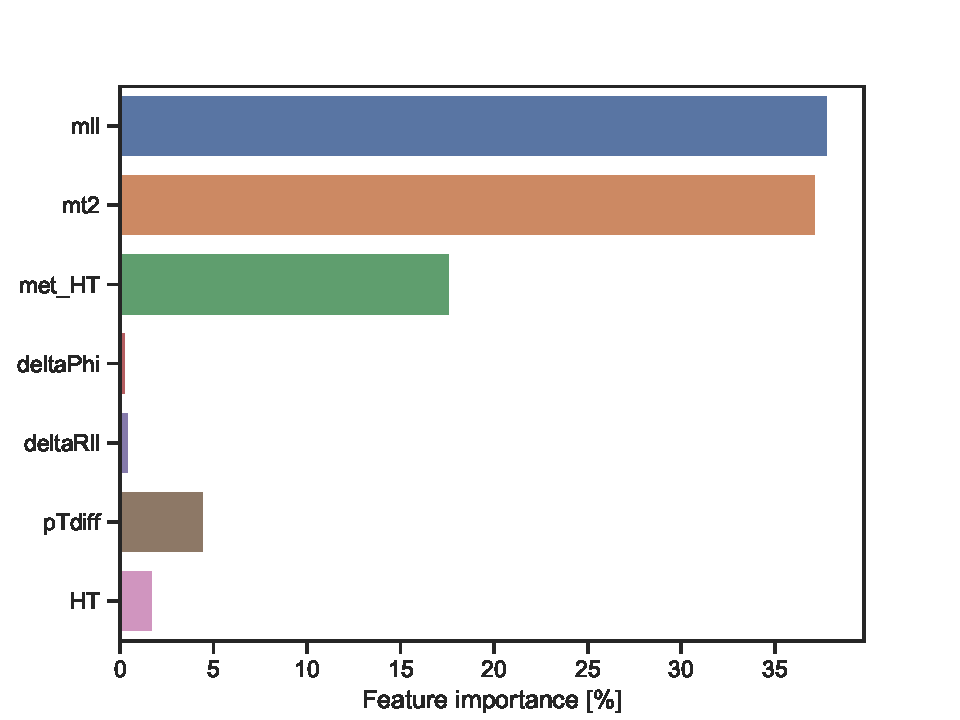
\includegraphics[width = \textwidth]{Figures/SlepSnu/BDT/High_level/Inter/featureImportance.pdf}
        \caption{}
        \label{fig:featSlepsnuLow}
    \end{subfigure}
    \begin{subfigure}[t!]{0.49\textwidth}
        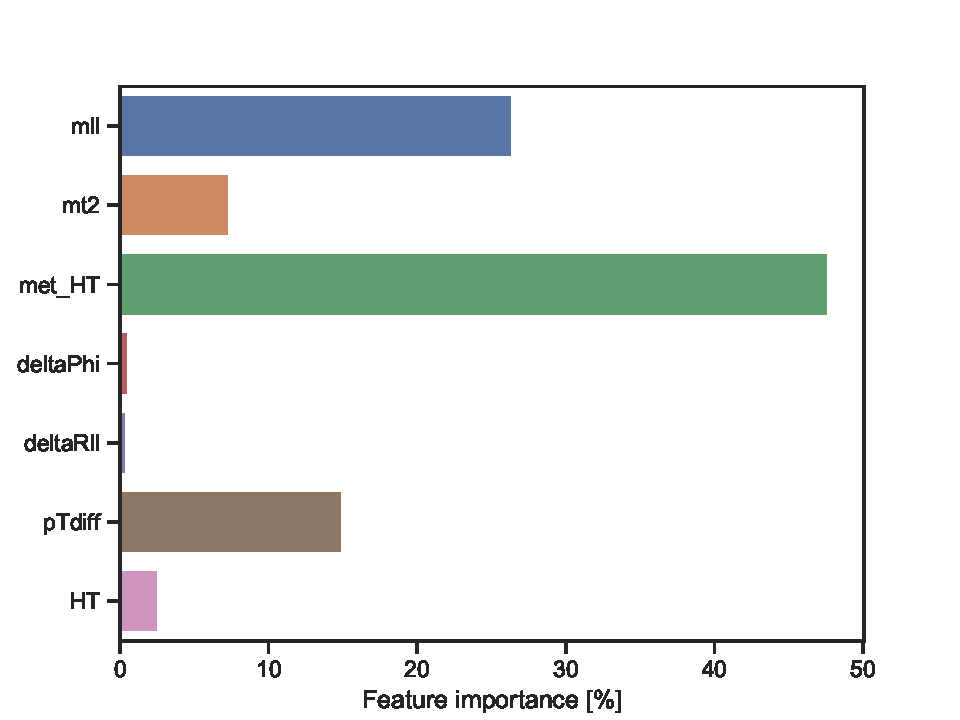
\includegraphics[width = \textwidth]{Figures/WW/BDT/High_level/Inter/featureImportance.pdf}
        \caption{}
        \label{fig:featWWLow}
    \end{subfigure}
    \begin{subfigure}[t!]{0.49\textwidth}
        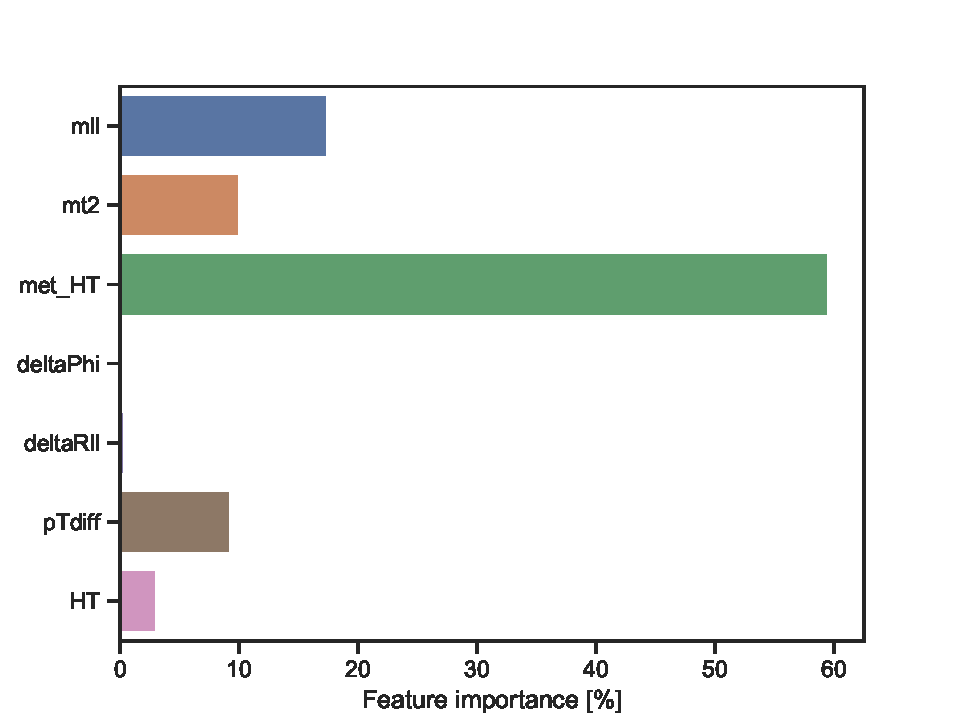
\includegraphics[width = \textwidth]{Figures/Mono_Z/ML/BDT/High_level/Inter/featureImportance.pdf}
        \caption{}
        \label{fig:featMonoZLow}
    \end{subfigure}
    \caption{}
    \label{fig:Non}
\end{figure}

\begin{figure}[H]
    \centering
    \begin{subfigure}[t!]{0.49\textwidth}
        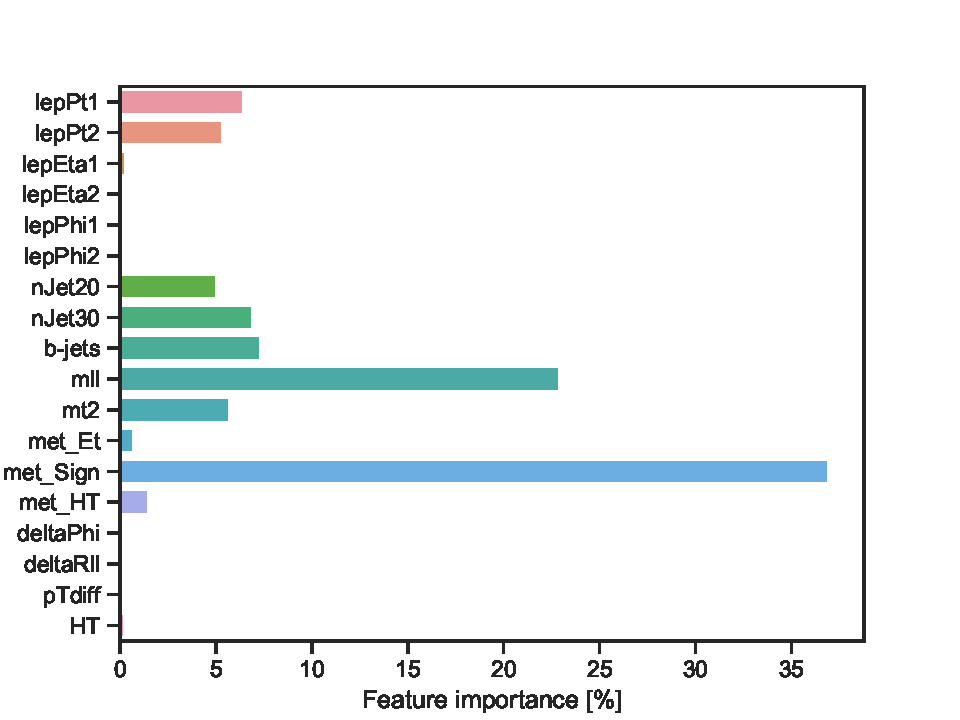
\includegraphics[width = \textwidth]{Figures/SlepSlep/ML/BDT/All_level/Inter/featureImportance.pdf}
        \caption{}
        \label{fig:featSlepslepLow}
    \end{subfigure}
    \begin{subfigure}[t!]{0.49\textwidth}
        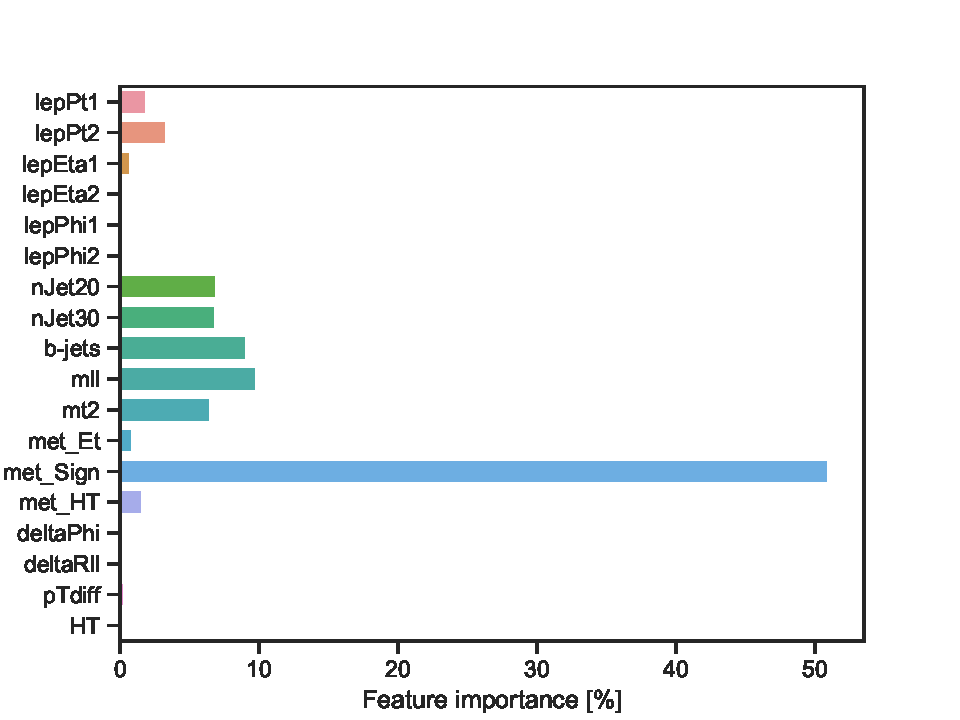
\includegraphics[width = \textwidth]{Figures/SlepSnu/BDT/All_level/Inter/featureImportance.pdf}
        \caption{}
        \label{fig:featSlepsnuLow}
    \end{subfigure}
    \begin{subfigure}[t!]{0.49\textwidth}
        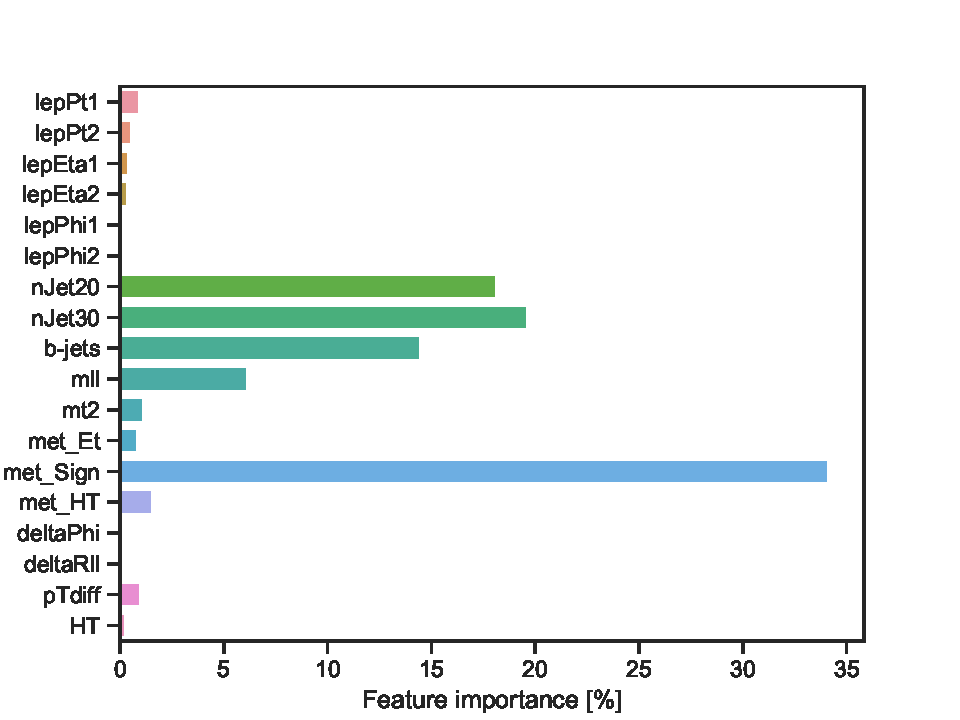
\includegraphics[width = \textwidth]{Figures/WW/BDT/All_level/Inter/featureImportance.pdf}
        \caption{}
        \label{fig:featWWLow}
    \end{subfigure}
    \begin{subfigure}[t!]{0.49\textwidth}
        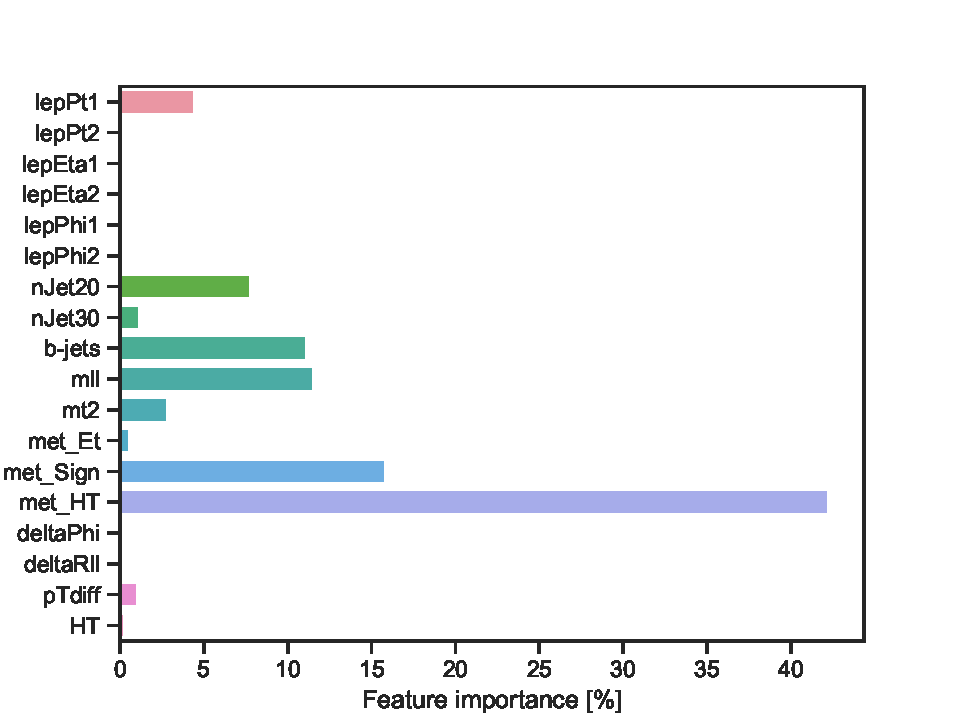
\includegraphics[width = \textwidth]{Figures/Mono_Z/ML/BDT/All_level/Inter/featureImportance.pdf}
        \caption{}
        \label{fig:featMonoZLow}
    \end{subfigure}
    \caption{}
    \label{fig:Non}
\end{figure}

\begin{figure}[H]
    \centering
    \begin{subfigure}[t!]{0.49\textwidth}
        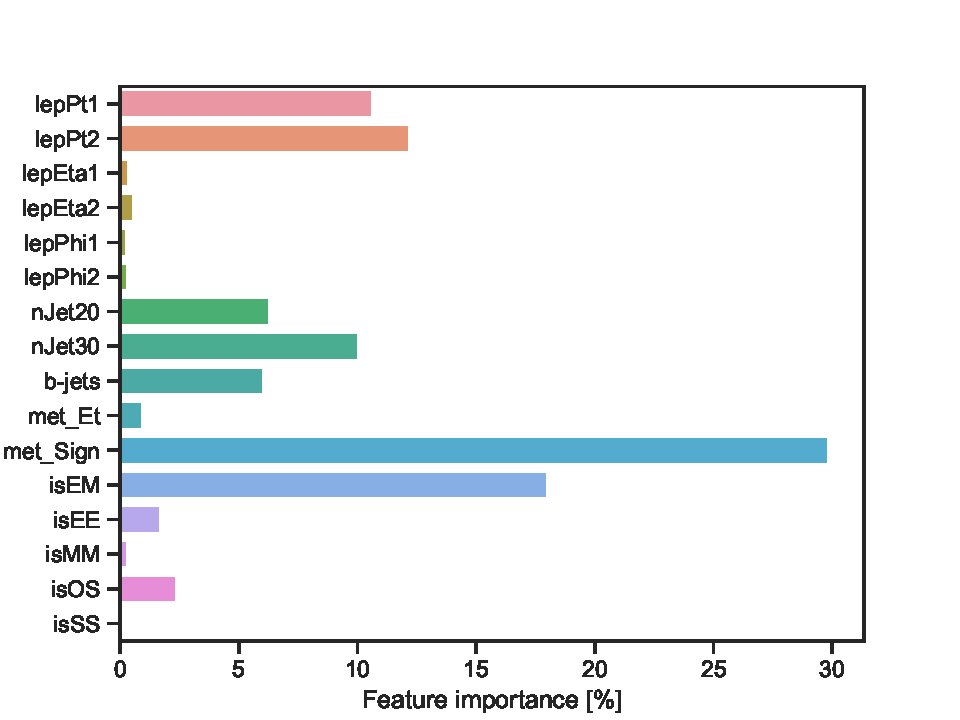
\includegraphics[width = \textwidth]{Figures/SlepSlep/ML/BDT/Low_level/Inter/featureImportance.pdf}
        \caption{}
        \label{fig:traintestscaled}
    \end{subfigure}
    \begin{subfigure}[t!]{0.49\textwidth}
        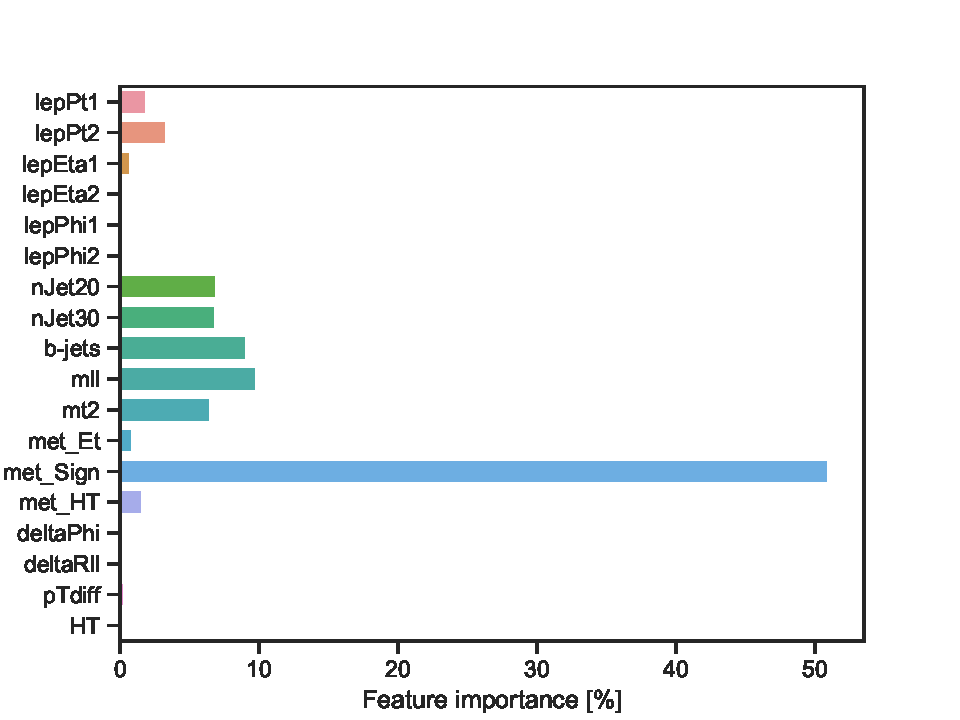
\includegraphics[width = \textwidth]{Figures/SlepSnu/BDT/All_level/Inter/featureImportance.pdf}
        \caption{}
        \label{fig:ROCBDTLow_low_level}
    \end{subfigure}
    \begin{subfigure}[t!]{0.49\textwidth}
        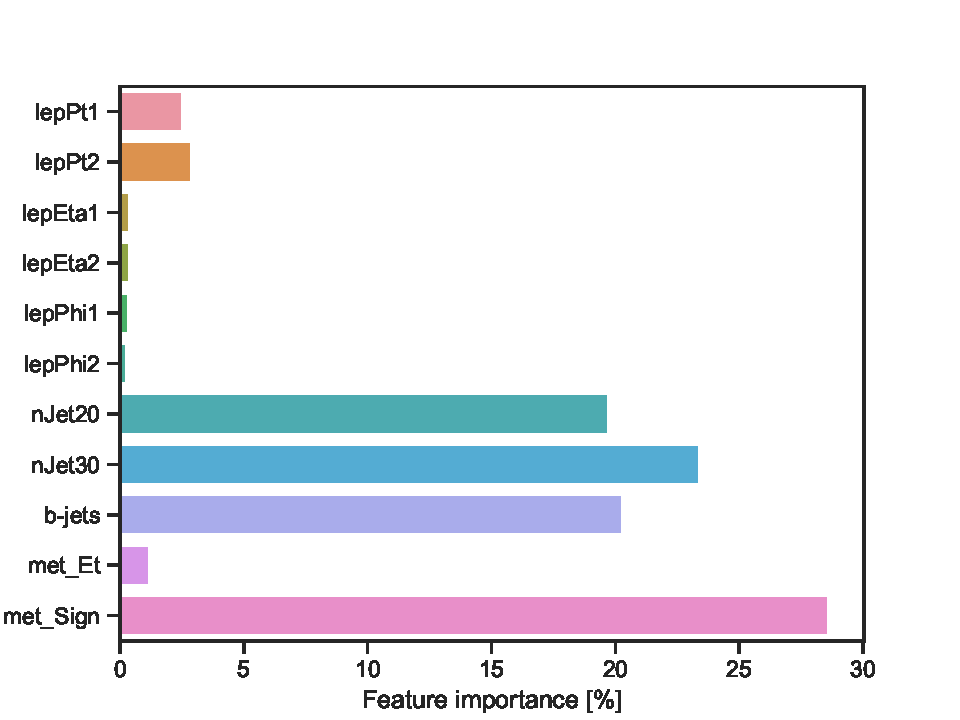
\includegraphics[width = \textwidth]{Figures/WW/BDT/Low_level/Inter/featureImportance.pdf}
        \caption{}
        \label{fig:traintestscaled}
    \end{subfigure}
    \begin{subfigure}[t!]{0.49\textwidth}
        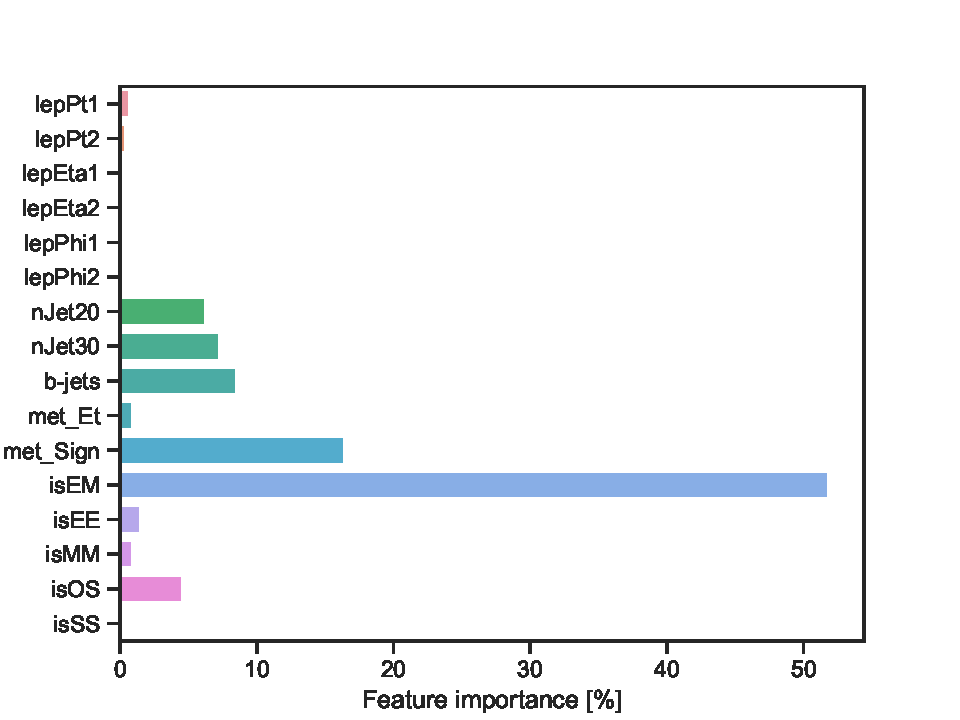
\includegraphics[width = \textwidth]{Figures/Mono_Z/ML/BDT/Low_level/Inter/featureImportance.pdf}
        \caption{}
        \label{fig:ROCBDTLow_low_level}
    \end{subfigure}
    \caption{}
    \label{fig:Non}
\end{figure}

\begin{figure}[H]
    \centering
    \begin{subfigure}[t!]{0.49\textwidth}
        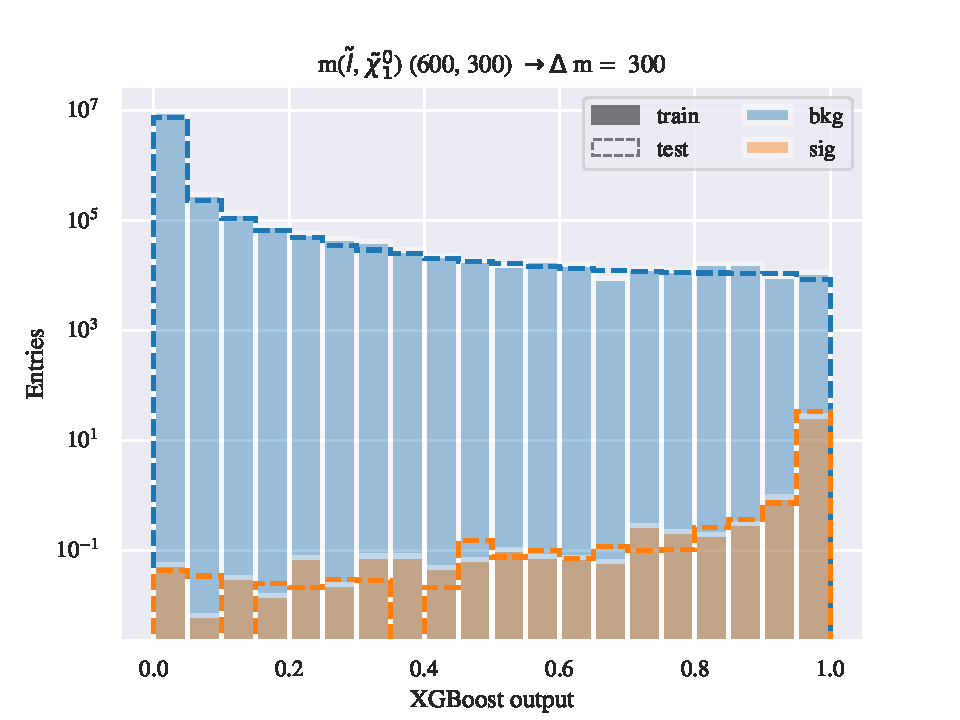
\includegraphics[width = \textwidth]{Figures/SlepSlep/ML/BDT/High_level/Inter/scaled_train_test_396014.pdf}
        \caption{}
        \label{fig:traintestscaled}
    \end{subfigure}
    \begin{subfigure}[t!]{0.49\textwidth}
        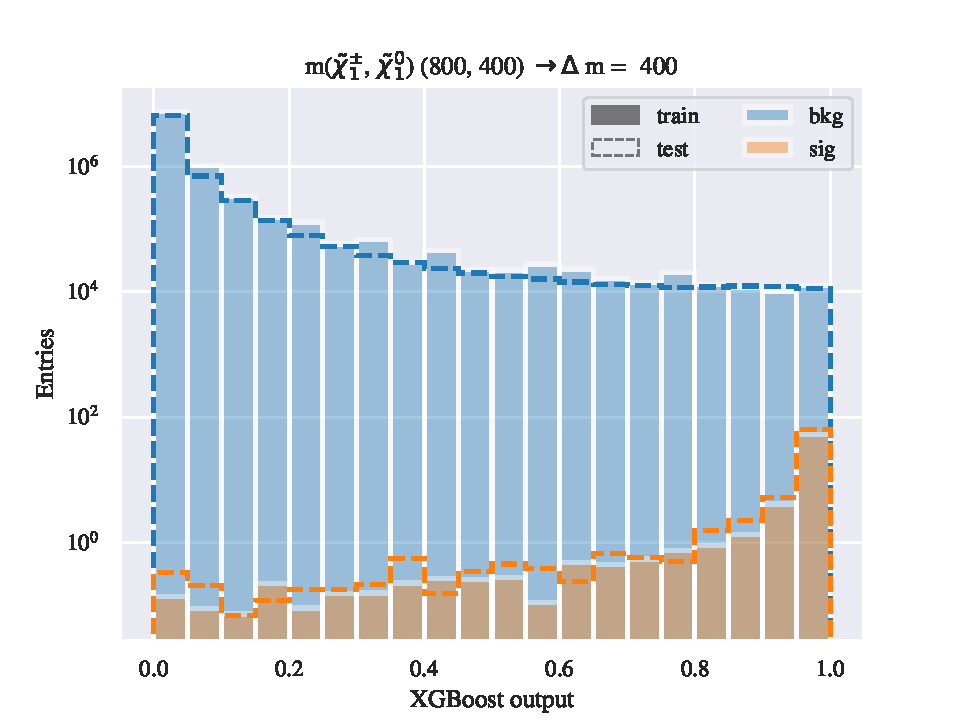
\includegraphics[width = \textwidth]{Figures/SlepSnu/BDT/Low_level/Inter/scaled_train_test_397150.pdf}
        \caption{}
        \label{fig:ROCBDTLow_low_level}
    \end{subfigure}
    \begin{subfigure}[t!]{0.49\textwidth}
        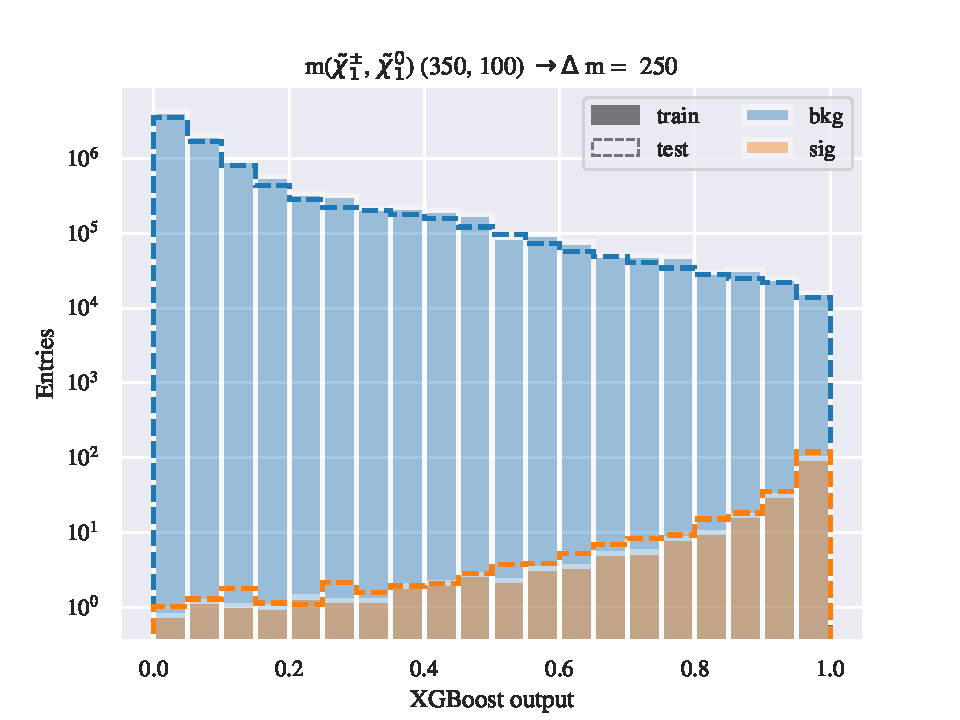
\includegraphics[width = \textwidth]{Figures/WW/BDT/Low_level/Inter/scaled_train_test_395320.pdf}
        \caption{}
        \label{fig:traintestscaled}
    \end{subfigure}
    \begin{subfigure}[t!]{0.49\textwidth}
        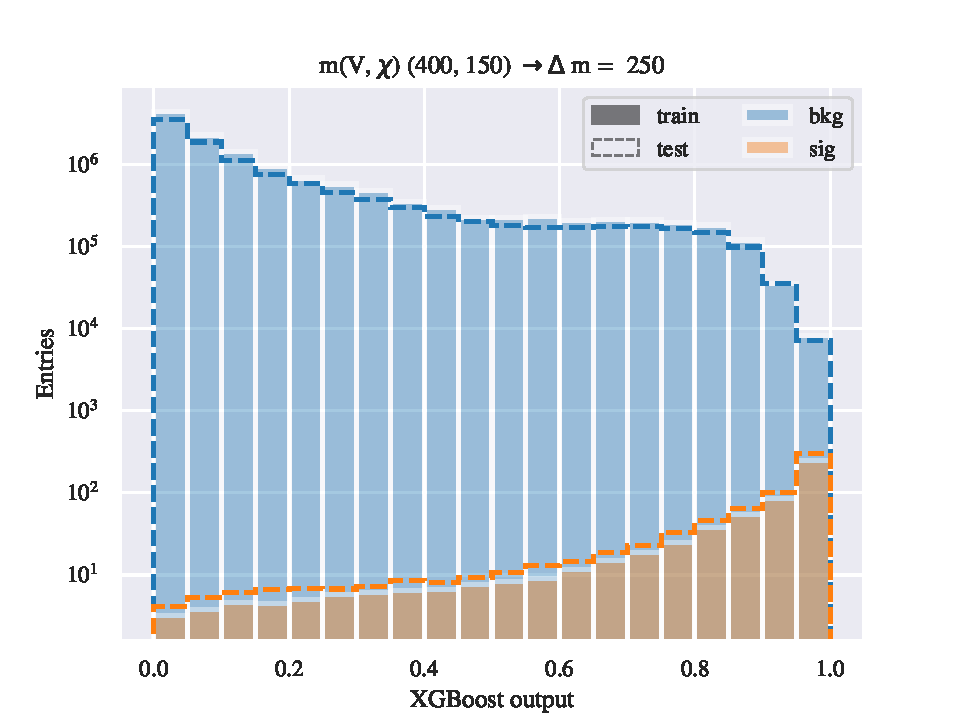
\includegraphics[width = \textwidth]{Figures/Mono_Z/ML/BDT/Low_level/Inter/scaled_train_test_310613.pdf}
        \caption{}
        \label{fig:ROCBDTLow_low_level}
    \end{subfigure}
    \caption{}
    \label{fig:Non}
\end{figure}

\subsubsection{High mass splittings}
\begin{figure}[H]
    \centering
    \begin{subfigure}[t!]{0.49\textwidth}
        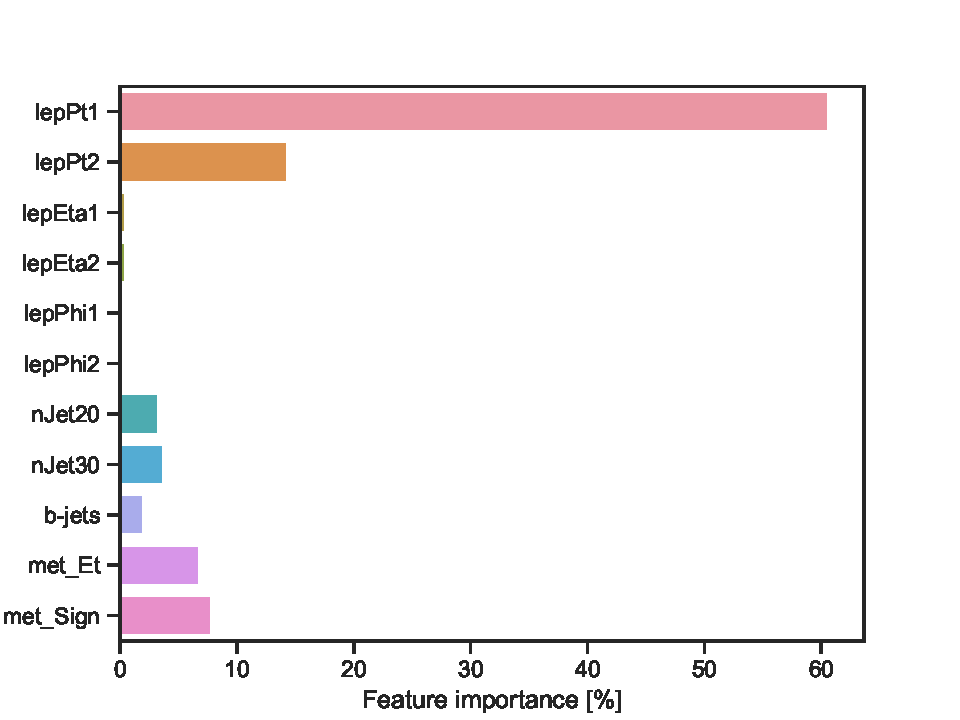
\includegraphics[width = \textwidth]{Figures/SlepSlep/ML/BDT/Low_level/High/featureImportance.pdf}
        \caption{}
        \label{fig:featSlepslepLow}
    \end{subfigure}
    \begin{subfigure}[t!]{0.49\textwidth}
        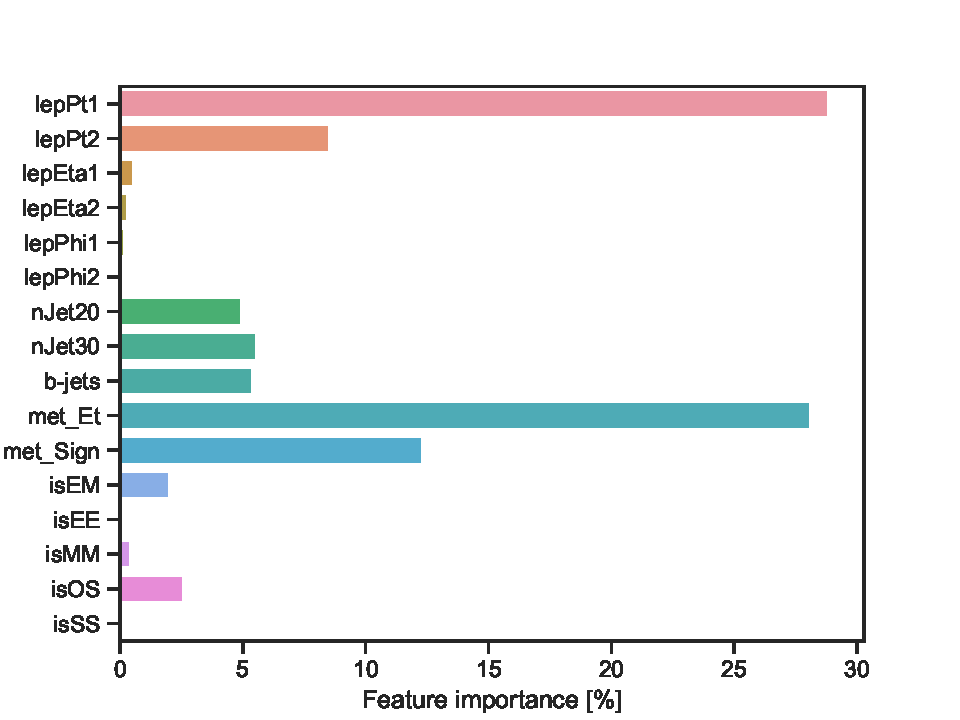
\includegraphics[width = \textwidth]{Figures/SlepSnu/BDT/Low_level/High/featureImportance.pdf}
        \caption{}
        \label{fig:featSlepsnuLow}
    \end{subfigure}
    \begin{subfigure}[t!]{0.49\textwidth}
        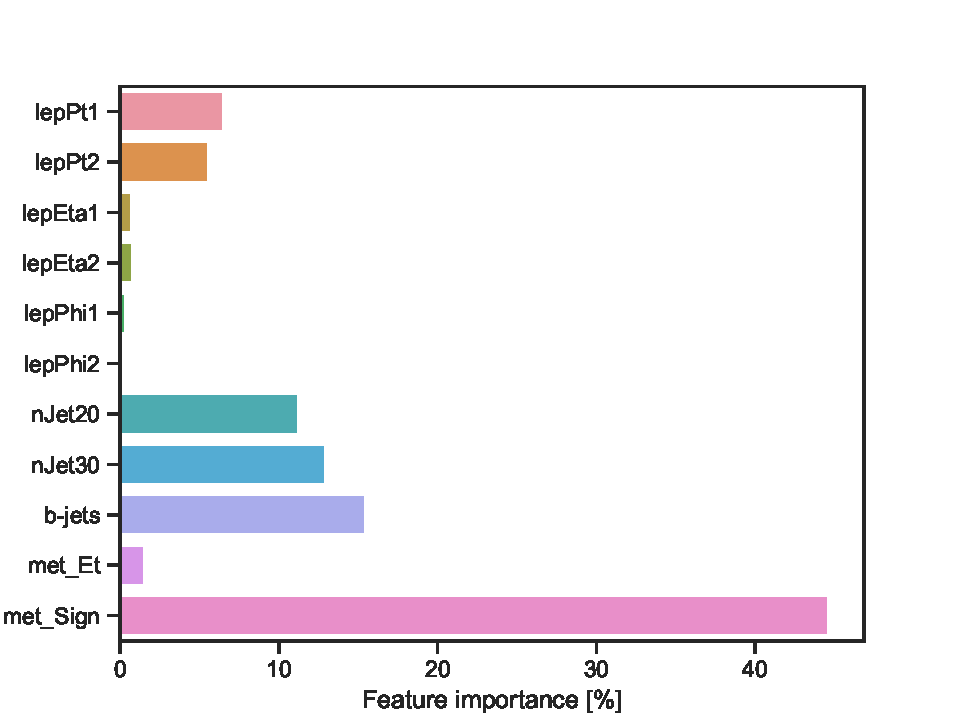
\includegraphics[width = \textwidth]{Figures/WW/BDT/Low_level/High/featureImportance.pdf}
        \caption{}
        \label{fig:featWWLow}
    \end{subfigure}
    \begin{subfigure}[t!]{0.49\textwidth}
        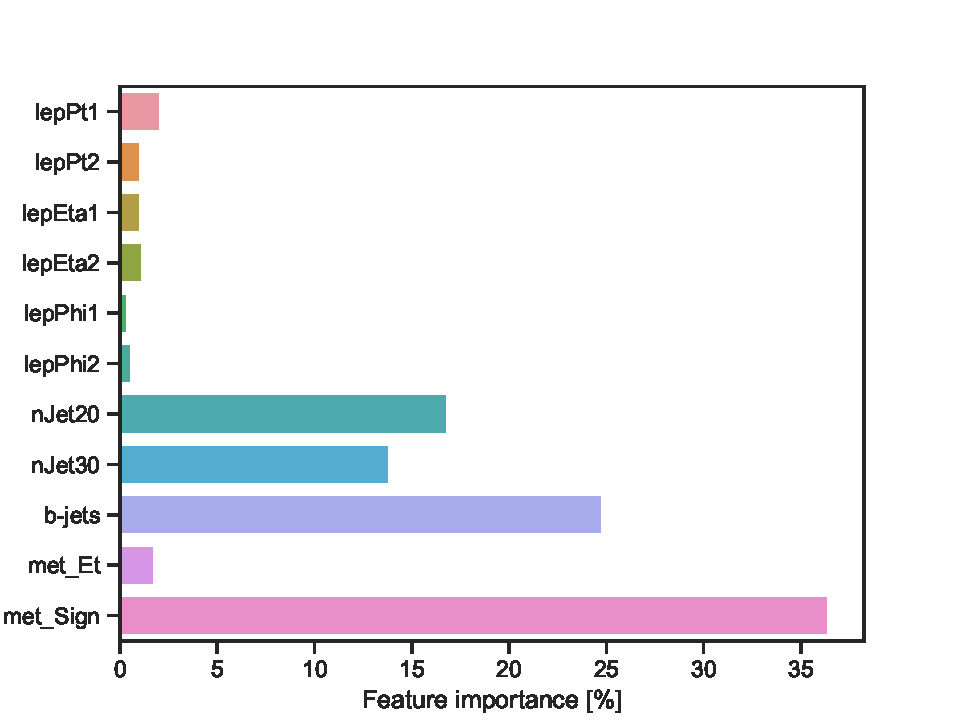
\includegraphics[width = \textwidth]{Figures/Mono_Z/ML/BDT/Low_level/High/featureImportance.pdf}
        \caption{}
        \label{fig:featMonoZLow}
    \end{subfigure}
    \caption{}
    \label{fig:Non}
\end{figure}

\begin{figure}[H]
    \centering
    \begin{subfigure}[t!]{0.49\textwidth}
        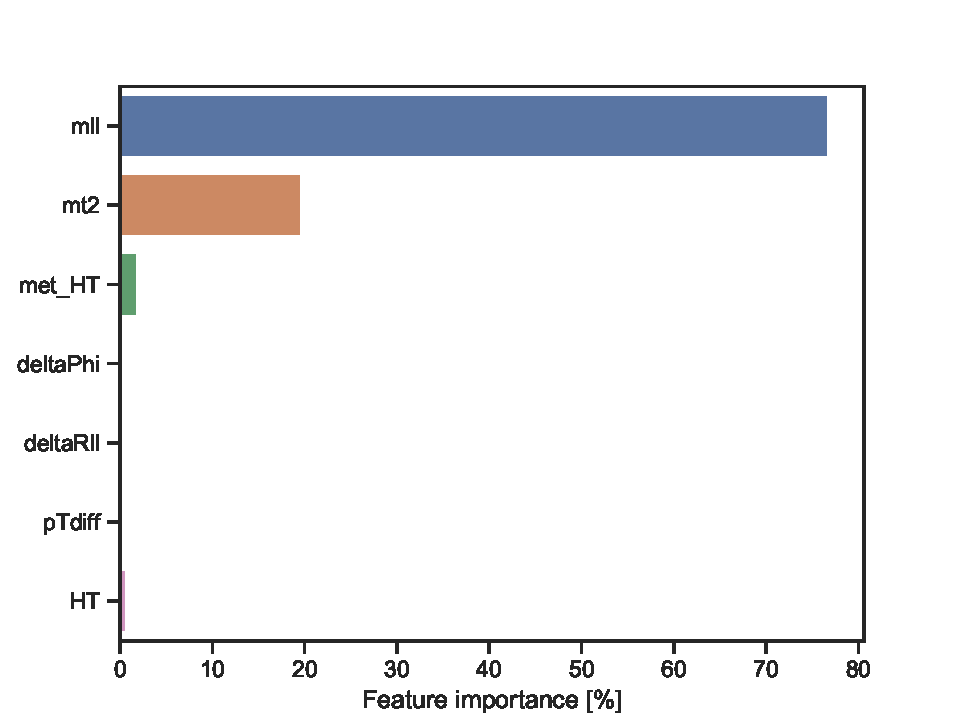
\includegraphics[width = \textwidth]{Figures/SlepSlep/ML/BDT/High_level/High/featureImportance.pdf}
        \caption{}
        \label{fig:featSlepslepLow}
    \end{subfigure}
    \begin{subfigure}[t!]{0.49\textwidth}
        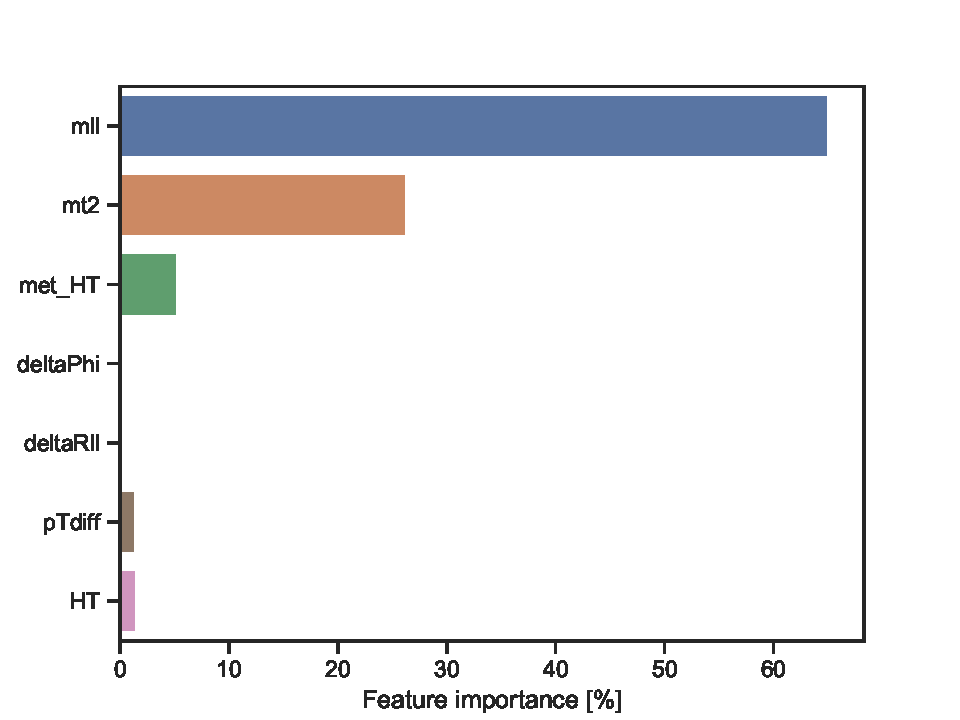
\includegraphics[width = \textwidth]{Figures/SlepSnu/BDT/High_level/High/featureImportance.pdf}
        \caption{}
        \label{fig:featSlepsnuLow}
    \end{subfigure}
    \begin{subfigure}[t!]{0.49\textwidth}
        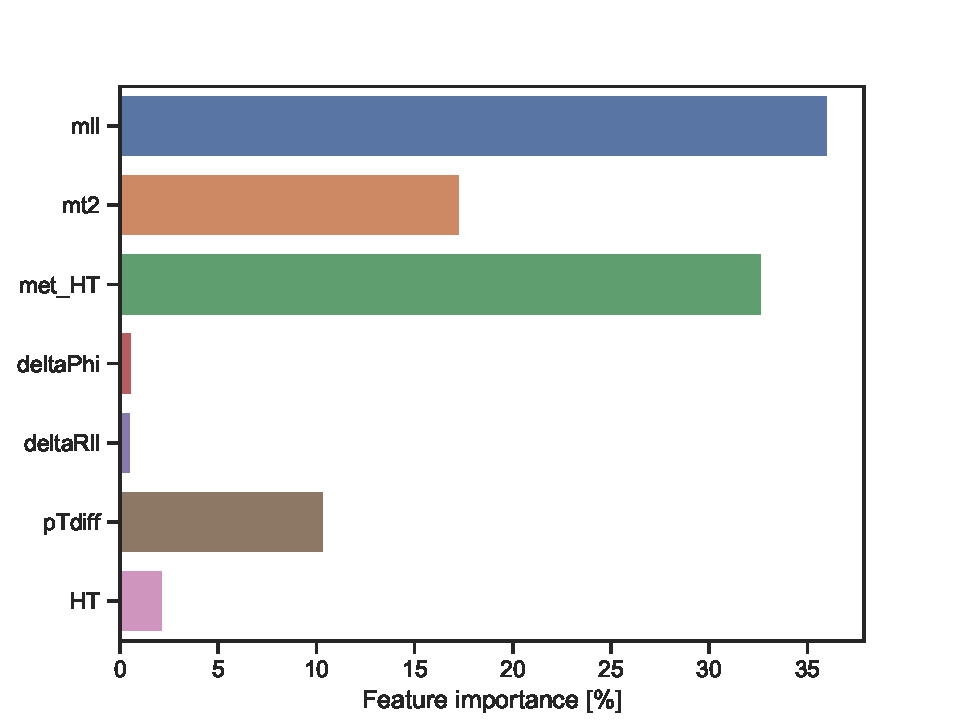
\includegraphics[width = \textwidth]{Figures/WW/BDT/High_level/High/featureImportance.pdf}
        \caption{}
        \label{fig:featWWLow}
    \end{subfigure}
    \begin{subfigure}[t!]{0.49\textwidth}
        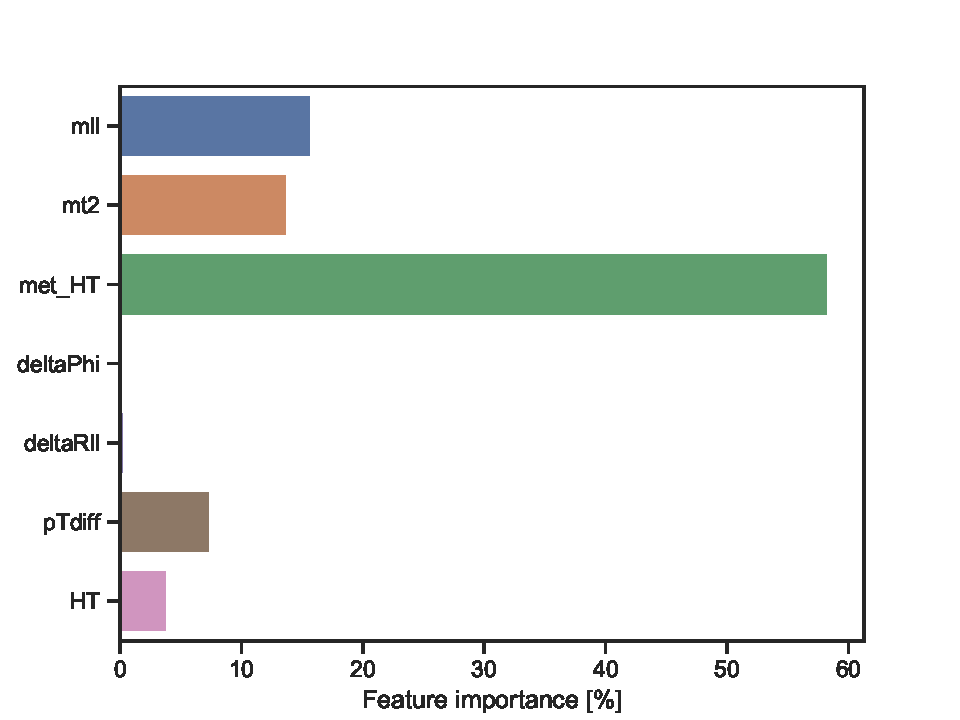
\includegraphics[width = \textwidth]{Figures/Mono_Z/ML/BDT/High_level/High/featureImportance.pdf}
        \caption{}
        \label{fig:featMonoZLow}
    \end{subfigure}
    \caption{}
    \label{fig:Non}
\end{figure}

\begin{figure}[H]
    \centering
    \begin{subfigure}[t!]{0.49\textwidth}
        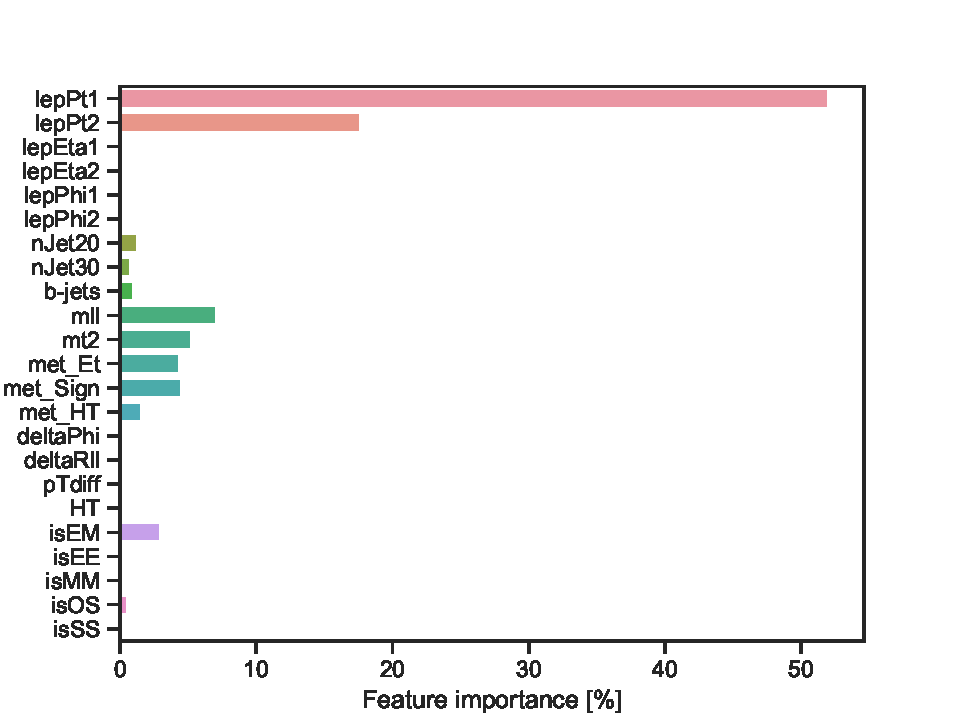
\includegraphics[width = \textwidth]{Figures/SlepSlep/ML/BDT/All_level/High/featureImportance.pdf}
        \caption{}
        \label{fig:featSlepslepLow}
    \end{subfigure}
    \begin{subfigure}[t!]{0.49\textwidth}
        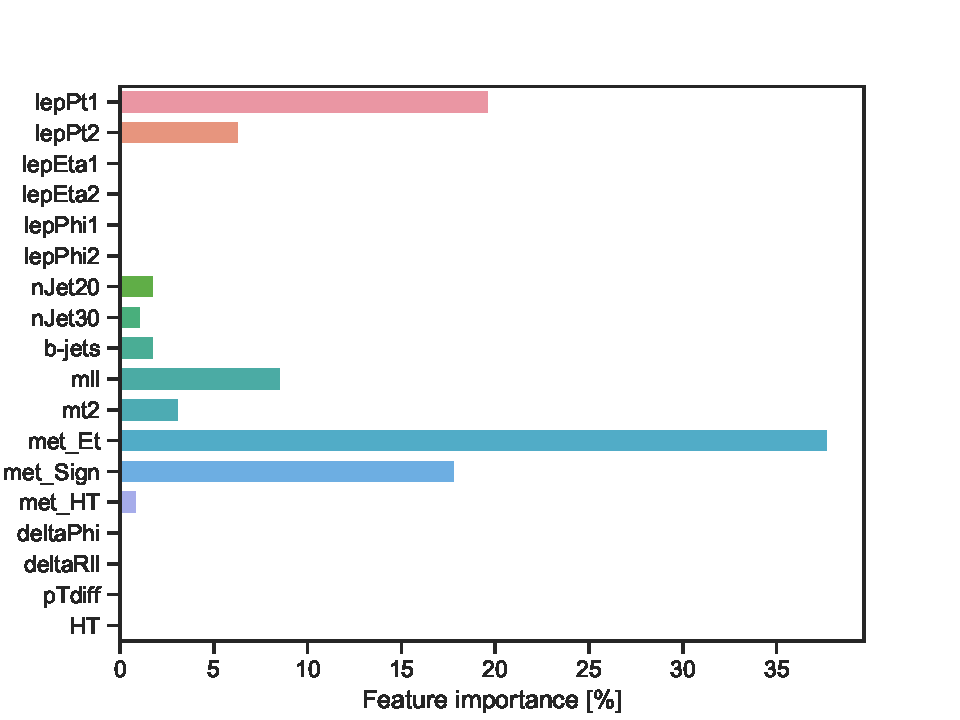
\includegraphics[width = \textwidth]{Figures/SlepSnu/BDT/All_level/High/featureImportance.pdf}
        \caption{}
        \label{fig:featSlepsnuLow}
    \end{subfigure}
    \begin{subfigure}[t!]{0.49\textwidth}
        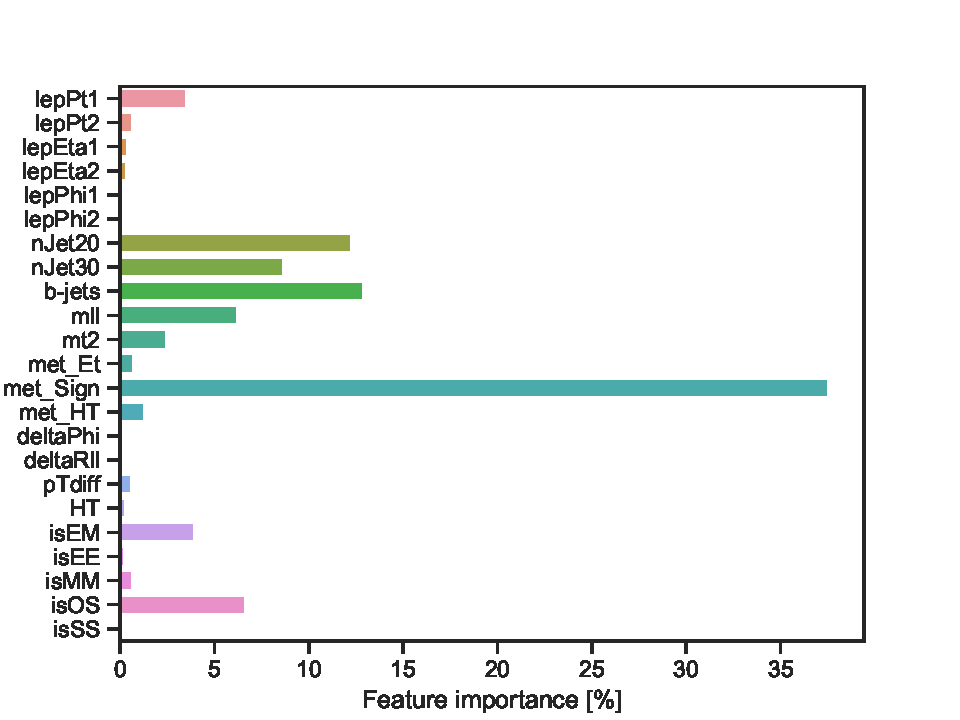
\includegraphics[width = \textwidth]{Figures/WW/BDT/All_level/High/featureImportance.pdf}
        \caption{}
        \label{fig:featWWLow}
    \end{subfigure}
    \begin{subfigure}[t!]{0.49\textwidth}
        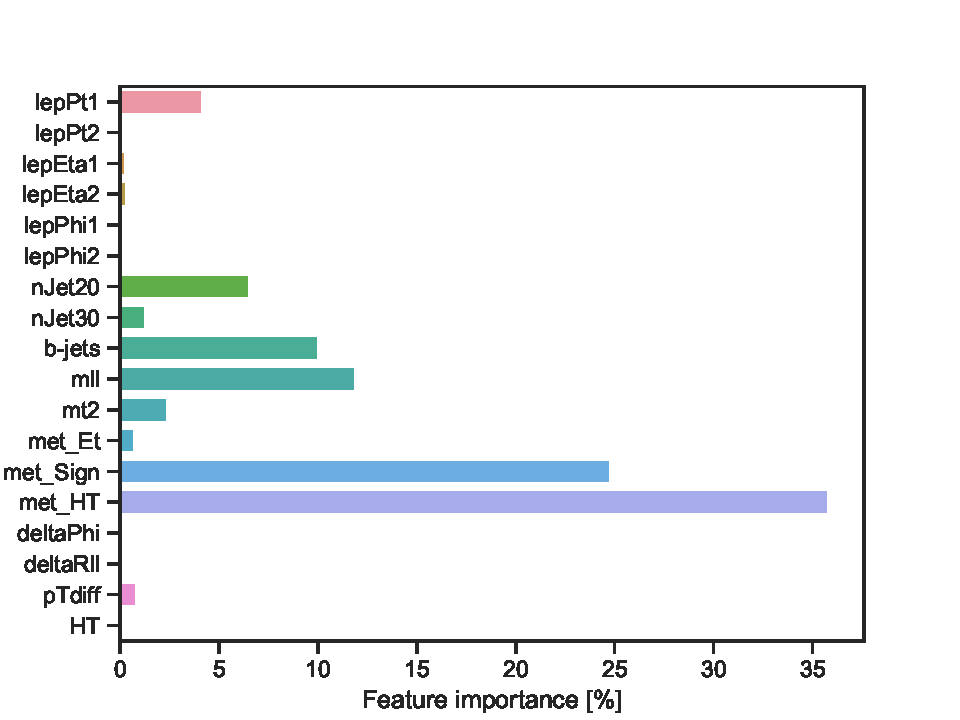
\includegraphics[width = \textwidth]{Figures/Mono_Z/ML/BDT/All_level/High/featureImportance.pdf}
        \caption{}
        \label{fig:featMonoZLow}
    \end{subfigure}
    \caption{}
    \label{fig:Non}
\end{figure}



\begin{figure}[H]
    \centering
    \begin{subfigure}[t!]{0.49\textwidth}
        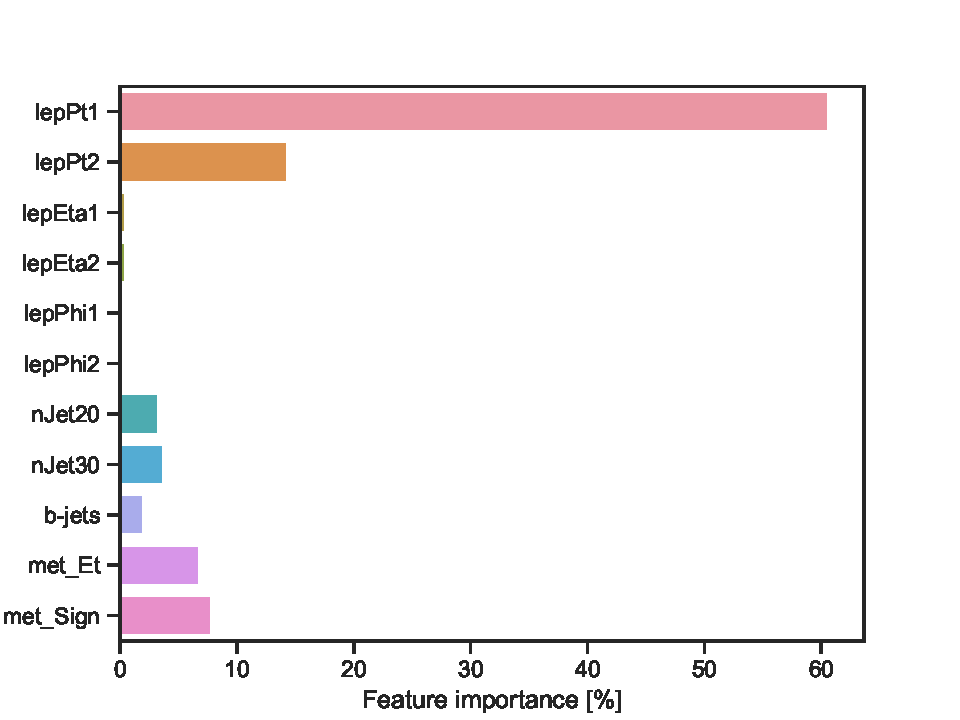
\includegraphics[width = \textwidth]{Figures/SlepSlep/ML/BDT/Low_level/High/featureImportance.pdf}
        \caption{}
        \label{fig:traintestscaled}
    \end{subfigure}
    \begin{subfigure}[t!]{0.49\textwidth}
        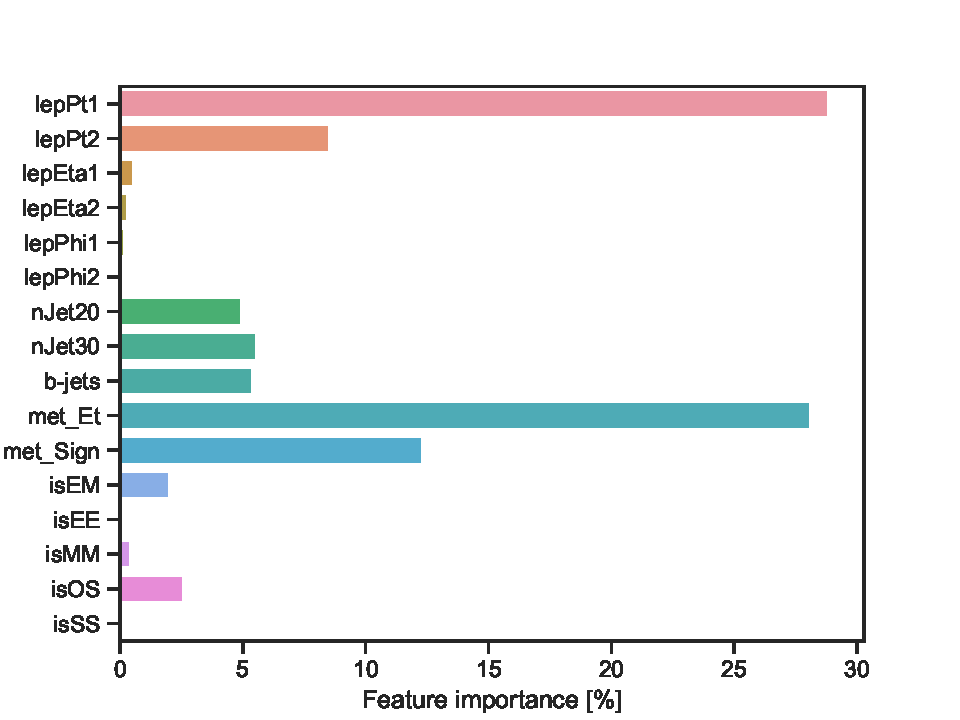
\includegraphics[width = \textwidth]{Figures/SlepSnu/BDT/Low_level/High/featureImportance.pdf}
        \caption{}
        \label{fig:ROCBDTLow_low_level}
    \end{subfigure}
    \begin{subfigure}[t!]{0.49\textwidth}
        \includegraphics[width = \textwidth]{Figures/WW/BDT/Low_level/High/featureImportance.pdf}
        \caption{}
        \label{fig:traintestscaled}
    \end{subfigure}
    \begin{subfigure}[t!]{0.49\textwidth}
        \includegraphics[width = \textwidth]{Figures/Mono_Z/ML/BDT/Low_level/High/featureImportance.pdf}
        \caption{}
        \label{fig:ROCBDTLow_low_level}
    \end{subfigure}
    \caption{}
    \label{fig:Non}
\end{figure}

\begin{figure}[H]
    \centering
    \begin{subfigure}[t!]{0.49\textwidth}
        \includegraphics[width = \textwidth]{Figures/SlepSlep/ML/BDT/High_level/High/scaled_train_test_396033.pdf}
        \caption{}
        \label{fig:traintestscaled}
    \end{subfigure}
    \begin{subfigure}[t!]{0.49\textwidth}
        \includegraphics[width = \textwidth]{Figures/SlepSnu/BDT/Low_level/High/scaled_train_test_397169.pdf}
        \caption{}
        \label{fig:ROCBDTLow_low_level}
    \end{subfigure}
    \begin{subfigure}[t!]{0.49\textwidth}
        \includegraphics[width = \textwidth]{Figures/WW/BDT/Low_level/High/scaled_train_test_395330.pdf}
        \caption{}
        \label{fig:traintestscaled}
    \end{subfigure}
    \begin{subfigure}[t!]{0.49\textwidth}
        \includegraphics[width = \textwidth]{Figures/Mono_Z/ML/BDT/Low_level/High/scaled_train_test_310617.pdf}
        \caption{}
        \label{fig:ROCBDTLow_low_level}
    \end{subfigure}
    \caption{}
    \label{fig:Non}
\end{figure}









\begin{figure}[H]
    \centering
    \begin{subfigure}[t!]{0.49\textwidth}
        \includegraphics[width = \textwidth]{Figures/Stacked/stackedplot_BDT_All_level_slepslep.pdf}
        \caption{Direct slepton production.}
        \label{fig:SlepslepNNLow}
    \end{subfigure}
    \begin{subfigure}[t!]{0.49\textwidth}
        \includegraphics[width = \textwidth]{Figures/Stacked/stackedplot_BDT_All_level_slepsnu.pdf}
        \caption{Chargino production via $\Tilde{l}/\Tilde{\nu}$.}
        \label{fig:SlepsnuNNLow}
    \end{subfigure}      
    \begin{subfigure}[t!]{0.49\textwidth}
        \includegraphics[width = \textwidth]{Figures/Stacked/stackedplot_BDT_All_level_WW.pdf}
        \caption{Chargino production via $W^\pm$.}
        \label{fig:WWNNLow}
    \end{subfigure}
    \begin{subfigure}[t!]{0.49\textwidth}
        \includegraphics[width = \textwidth]{Figures/Stacked/stackedplot_BDT_All_level_monoZ.pdf}
        \caption{Mono-Z.}
        \label{fig:MonoZNNLow}
    \end{subfigure}
    \caption{Test vs train for low mass splittings done with the NN. Here the test set is scaled up to match the number of training events.}
    \label{fig:AllLowNN}
\end{figure}


\begin{figure}[H]
    \centering
    \begin{subfigure}[t!]{0.49\textwidth}
        \includegraphics[width = \textwidth]{Figures/Stacked/stackedplot_BDT_Low_level_slepslep.pdf}
        \caption{Direct slepton production.}
        \label{fig:SlepslepNNLow}
    \end{subfigure}
    \begin{subfigure}[t!]{0.49\textwidth}
        \includegraphics[width = \textwidth]{Figures/Stacked/stackedplot_BDT_Low_level_slepsnu.pdf}
        \caption{Chargino production via $\Tilde{l}/\Tilde{\nu}$.}
        \label{fig:SlepsnuNNLow}
    \end{subfigure}      
    \begin{subfigure}[t!]{0.49\textwidth}
        \includegraphics[width = \textwidth]{Figures/Stacked/stackedplot_BDT_Low_level_WW.pdf}
        \caption{Chargino production via $W^\pm$.}
        \label{fig:WWNNLow}
    \end{subfigure}
    \begin{subfigure}[t!]{0.49\textwidth}
        \includegraphics[width = \textwidth]{Figures/Stacked/stackedplot_BDT_Low_level_monoZ.pdf}
        \caption{Mono-Z.}
        \label{fig:MonoZNNLow}
    \end{subfigure}
    \caption{Test vs train for low mass splittings done with the NN. Here the test set is scaled up to match the number of training events.}
    \label{fig:AllLowNN}
\end{figure}

\begin{figure}[H]
    \centering
    \begin{subfigure}[t!]{0.49\textwidth}
        \includegraphics[width = \textwidth]{Figures/Stacked/stackedplot_BDT_High_level_slepslep.pdf}
        \caption{Direct slepton production.}
        \label{fig:SlepslepNNLow}
    \end{subfigure}
    \begin{subfigure}[t!]{0.49\textwidth}
        \includegraphics[width = \textwidth]{Figures/Stacked/stackedplot_BDT_High_level_slepsnu.pdf}
        \caption{Chargino production via $\Tilde{l}/\Tilde{\nu}$.}
        \label{fig:SlepsnuNNLow}
    \end{subfigure}      
    \begin{subfigure}[t!]{0.49\textwidth}
        \includegraphics[width = \textwidth]{Figures/Stacked/stackedplot_BDT_High_level_WW.pdf}
        \caption{Chargino production via $W^\pm$.}
        \label{fig:WWNNLow}
    \end{subfigure}
    \begin{subfigure}[t!]{0.49\textwidth}
        \includegraphics[width = \textwidth]{Figures/Stacked/stackedplot_BDT_High_level_monoZ.pdf}
        \caption{Mono-Z.}
        \label{fig:MonoZNNLow}
    \end{subfigure}
    \caption{Test vs train for low mass splittings done with the NN. Here the test set is scaled up to match the number of training events.}
    \label{fig:AllLowNN}
\end{figure}








